\documentclass[main.tex]{subfiles}
\newcommand{\DiagramaEscala}{0.9}
\begin{document}




% Sección 1: Introducción
\section{Introducción a la Energia}
\begin{frame}{Definición de Energía}
  \justifying
  El término \textbf{Energía} tiene múltiples significados según el contexto. En el lenguaje cotidiano, se asocia con vitalidad o estados emocionales, mientras que en ciencias y tecnología se usa en expresiones como \textbf{crisis energética} o "\textbf{alimentos energéticos}. Aunque sus efectos son bien conocidos, su verdadera naturaleza sigue siendo un misterio. En física, la energía se define como una propiedad de los cuerpos o sistemas que les permite transformarse y modificar su estado, así como generar cambios en otros sistemas. En esencia, es la capacidad de producir transformaciones, sin importar si estas ocurren o no.
  
  La energía es la capacidad de un sistema para realizar trabajo. Se manifiesta en diversas formas y puede transferirse o transformarse de una a otra.
\end{frame}




% Sección 2: Trabajo y Energía
%\section{Trabajo y Energía}
\begin{frame}{Concepto de Trabajo}
  \justifying
  En física, el trabajo se define como el producto escalar de una fuerza por un desplazamiento:
  \begin{equation}
    W = \vec{F} \cdot \vec{\Delta S}
  \end{equation}
  donde $W$ es el trabajo, $\vec{F}$ la fuerza aplicada y $\vec{\Delta S}$ el desplazamiento.

  \justifying
  El trabajo se mide en julios (J), definidos como:
  \begin{equation}
    1 J = 1 N \cdot 1 m
  \end{equation}
  Un julio equivale al trabajo realizado cuando una fuerza de un newton desplaza un objeto un metro en la misma dirección de la fuerza.
\end{frame}

\begin{frame}{Relación entre Trabajo y Energía}
  \justifying
  Tradicionalmente, la energía se define como la capacidad de realizar trabajo. Ambas magnitudes comparten la misma unidad de medida: el julio (J).
  \begin{itemize}
    \item Aunque se dice que la energía se transforma en trabajo, en realidad el trabajo es un proceso mediante el cual la energía se transfiere de un sistema a otro.
    \item Un ejemplo es el levantamiento de una masa $m$ a una altura $h$, donde la energía almacenada en los músculos de la persona se transfiere a energía potencial gravitatoria del objeto:
    \begin{equation}
      W = mgh
    \end{equation}
  \end{itemize}
\end{frame}

\begin{frame}{El Trabajo como un Proceso de Transferencia de Energía}
  \justifying
  El trabajo no es una forma de energía en sí misma, ni se conserva, sino que es un mecanismo mediante el cual los cuerpos intercambian energía. Otro proceso de transferencia de energía es el calor.
  \begin{itemize}
    \item Ejemplo: Cuando una persona empuja un objeto, la energía química en los músculos se transforma en energía cinética del objeto en movimiento.
  \end{itemize}
\end{frame}




% Sección 3: Potencia
%\section{Potencia}
\begin{frame}{Definición de Potencia}
  \justifying
  La potencia es la cantidad de trabajo realizado por unidad de tiempo. Matemáticamente, se expresa como:
  \begin{equation}
    P = \frac{W}{t}
  \end{equation}
  donde $P$ es la potencia, $W$ el trabajo realizado y $t$ el tiempo empleado.

  La unidad de la potencia en el Sistema Internacional es el vatio (W), definido como:
  \begin{equation}
    1 W = \frac{1 J}{1 s}
  \end{equation}
  Esto significa que un vatio equivale a realizar un julio de trabajo en un segundo.
\end{frame}




\begin{frame}{Ejemplo de Potencia}
  \justifying
  En la Figura se observa que la persona más corpulenta es capaz de elevar una masa $m$, de peso $P$, más rápidamente que la menos corpulenta. En términos físicos, la primera ejecuta el mismo trabajo que la segunda ($W = mgh$), pero en menor tiempo, por lo que tiene mayor potencia.
  \begin{figure}
    \centering
    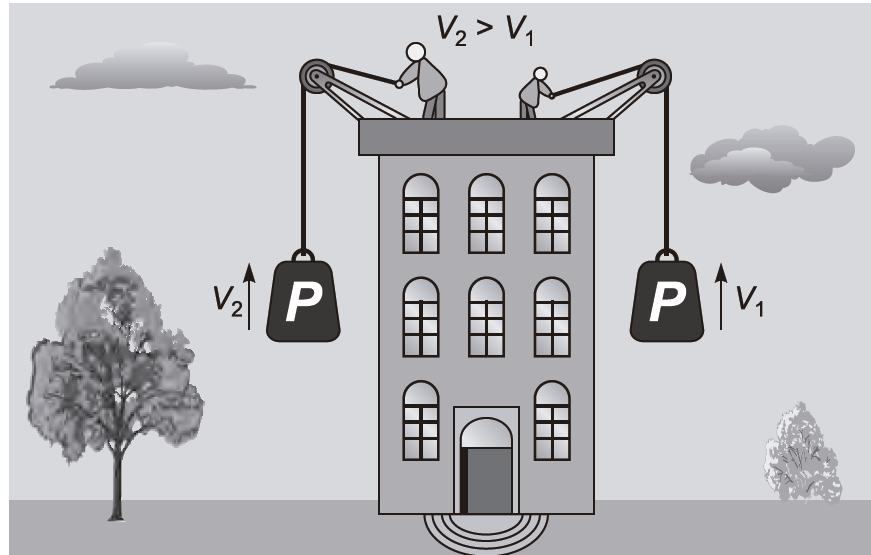
\includegraphics[width=0.4\linewidth]{img/figura_1_potencia.png} % Imagen de referencia
    \caption{Comparación de potencia entre dos personas levantando una masa.}
  \end{figure}
\end{frame}




\begin{frame}{Conversión de Potencia y Energía}
\small
\renewcommand{\arraystretch}{1.1}
\setlength{\tabcolsep}{4pt}
\centering
\begin{tabular}{|l l|l l|}
    \hline
    \multicolumn{2}{|l|}{\textbf{Potencia:}} & \multicolumn{2}{l|}{\textbf{Energía:}} \\
    \hline
    1 CV & = 0,76 kW & 1 kcal & = 4,186 kJ \\
    1 HP & = 0,746 kW & 1 BTU & = 1.055 J \\
    & & & \textit{(British Thermal Unit)} \\
    \hline
    \multicolumn{4}{|l|}{\footnotesize 1 Tep $=$ 42.000 MJ $=$ 11.600 kWh} \\
    \multicolumn{4}{|l|}{\footnotesize (1 Tn petróleo $\approx$ 7,3 barriles)} \\
    \multicolumn{4}{|l|}{\footnotesize 1 Tec $=$ 28.000 MJ $=$ 7.500 kWh} \\
    \multicolumn{4}{|l|}{\footnotesize 1.000 m$^3$ gas $\approx$ 6,81 barriles de petróleo} \\
    \multicolumn{4}{|l|}{\footnotesize 1.000 m$^3$ gas $\approx$ 0,9 tep} \\
    \multicolumn{4}{|l|}{\footnotesize 1 Termia $=$ $10^{-4}$ Tep $=$ $10^3$ kcal} \\
    \hline
    \multicolumn{4}{|l|}{\tiny (Tep $=$ Tn equivalente de petróleo)} \\
    \multicolumn{4}{|l|}{\tiny (1 barril $=$ 158,9 litros)} \\
    \multicolumn{4}{|l|}{\tiny (Tec $=$ Tn equivalente de carbón)} \\
    \hline
\end{tabular}
\end{frame}



\begin{frame}
    \frametitle{Manifestaciones de la energía}
    \framesubtitle{Energía gravitacional}

    \textbf{Energía gravitacional}: Es la energía que se manifiesta por la atracción de dos masas entre sí, sean cuerpos celestes, masas cualesquiera o incluso neutrones.

    \vspace{0.1cm}
    \textbf{Campo gravitatorio}: Cada masa crea un campo gravitatorio a su alrededor, atrayendo a cualquier otra masa que caiga en su campo de acción.

    \vspace{0.1cm}
    La fuerza de atracción es proporcional al producto de las masas e inversamente proporcional al cuadrado de la distancia entre ellas:

    \begin{equation}
        F = k \cdot \frac{M_1 \cdot M_2}{r^2}
    \end{equation}

    \centering
    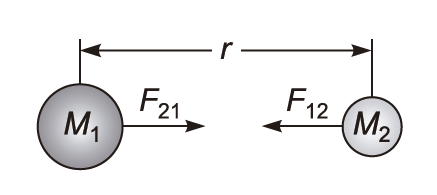
\includegraphics[width=0.2\linewidth]{img/Fuerzas_gravitatorias.png}
    
    \small{\textbf{Figura 1.3.} Fuerzas gravitatorias.}
\end{frame}

\begin{frame}
    \frametitle{Energía Potencial Gravitatoria}

    \textbf{Definición:} Es la atracción de la masa de la Tierra sobre cualquier otra masa cercana (ej. satélite, persona, etc.).

    \vspace{0.2cm}
    Se expresa como:

    \begin{equation}
        \text{Energía} = \text{fuerza} \times \text{distancia}
    \end{equation}

    \begin{equation}
        \text{Energía potencial} = \text{peso} \times \text{altura} = m \cdot g \cdot h
    \end{equation}

    Donde:
    \begin{itemize}
        \item $m$ en kg (kilogramos)
        \item $h$ en m (metros)
        \item $g$ en m/s$^2$ (aceleración de la gravedad)
    \end{itemize}

    \vspace{0.2cm}
    La energía se expresa en \textbf{Julios (J)}.
\end{frame}


\begin{frame}
    \frametitle{Energía Cinética}

    \textbf{Definición:} Es la energía implícita en una masa en movimiento. 
    Para una masa $m$ que se desplaza a la velocidad $v$, la energía cinética es:

    \begin{equation}
        W = \frac{1}{2} m \cdot v^2
    \end{equation}

    \vspace{0.1cm}
    \textbf{Unidades:} 
    \begin{itemize}
        \item $W$ en julios (J).
        \item $m$ en kilogramos (kg).
        \item $v$ en metros por segundo (m/s).
    \end{itemize}

    \centering
    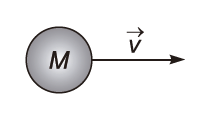
\includegraphics[width=0.2\linewidth]{img/energia_cinetica.png}

    \small{\textbf{Figura 1.4.} Energía cinética.}
\end{frame}

% Diapositiva 2: Energía Cinética en los gases
\begin{frame}
    \frametitle{Energía Cinética en Gases}

    \begin{columns}
        % Columna izquierda con el texto
        \column{0.6\textwidth}
        Un caso particular de la energía cinética es la \textbf{energía térmica}. 

        \vspace{0.3cm}
        \textbf{Movimiento de moléculas:}
        \begin{itemize}
            \item En los gases, las moléculas tienen total libertad de movimiento.
            \item Al aumentar la energía, se mueven más rápido y el gas se calienta.
        \end{itemize}

        % Columna derecha con la imagen
        \column{0.4\textwidth}
        \centering
        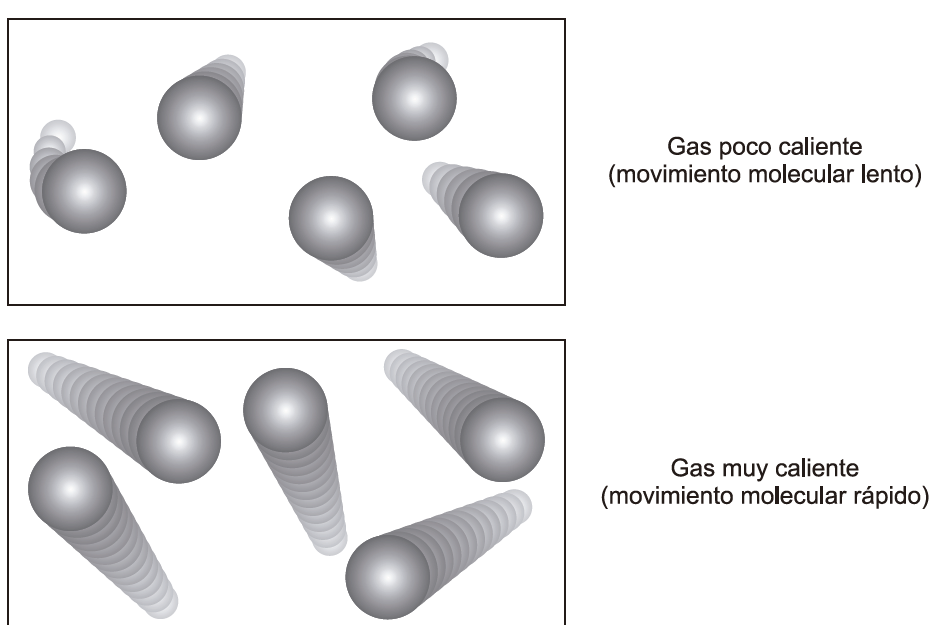
\includegraphics[width=\linewidth]{img/energia_cinetica_gases.png}

        \small{\textbf{Figura 1.5.} Energía cinética en gases.}
    \end{columns}

\end{frame}

% Diapositiva 3: Transferencia de Energía
\begin{frame}
    \frametitle{Transferencia de Energía}

    \textbf{Sensación de Calor:}
    \begin{itemize}
        \item Se debe al choque de las moléculas del aire con la piel.
        \item Aumenta la vibración molecular en la piel, generando sensación térmica.
    \end{itemize}

    \vspace{0.3cm}
    \textbf{Casos Especiales:}
    \begin{itemize}
        \item Un metal caliente transfiere energía cinética a la piel, aumentando la vibración molecular.
        \item La energía cinética se transfiere de partículas más rápidas a más lentas.
        \item A temperatura de $0$ Kelvin (\textbf{Cero Absoluto} = $-273^{\circ}$C), las moléculas no se mueven.
    \end{itemize}

    \vspace{0.3cm}
    \textbf{Conclusión:} La energía térmica es un caso especial de la energía cinética, que depende del movimiento molecular.

\end{frame}


\begin{frame}
    \frametitle{Energía Electroestática}

    La \textbf{energía electrostática} se manifiesta por la atracción o repulsión de dos cargas eléctricas. 

  %  \vspace{0.1cm}
  %  \textbf{Principios:}
    \begin{itemize}
        \item Cargas de \textbf{signo contrario} se atraen.
        \item Cargas de \textbf{mismo signo} se repelen.
        \item La fuerza es proporcional al producto de las cargas e inversamente proporcional al cuadrado de la distancia.
    \end{itemize}

    \begin{equation}
        F = k \cdot \frac{q_1 \cdot q_2}{r^2}
    \end{equation}

    \begin{columns}
        \column{0.8\textwidth}
        %\textbf{Campo Eléctrico:}
        \begin{itemize}
            \item Un cuerpo cargado genera un \textbf{campo eléctrico} que atrae o repele otras cargas cercanas.
            \item Se relaciona con la \textbf{energía química}, ya que mantiene unidos los átomos en las moléculas.
        \end{itemize}

        \column{0.5\textwidth}
        
        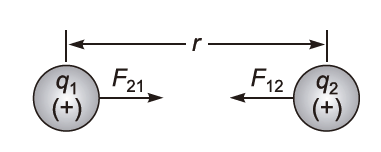
\includegraphics[width=0.5\linewidth]{img/fuerzas electrostaticas.png}

        %\small{\textbf{Figura 1.6.} Fuerzas electrostáticas.}
    \end{columns}
\end{frame}

\begin{frame}
    \frametitle{Relación con la Energía Química}

    \textbf{Ejemplo: Combustión de un Combustible}
    \begin{itemize}
        \item La energía química almacenada en los enlaces se transforma en otros tipos de energía.
        \item Se redistribuyen las cargas eléctricas en los productos de la reacción.
        \item Se generan \textbf{movimientos vibratorios} en las moléculas, aumentando la temperatura.
    \end{itemize}

    \vspace{0.3cm}
    \textbf{Conclusión:} La energía electrostática juega un papel fundamental en los procesos químicos y térmicos, al influir en la estabilidad de las moléculas y la transferencia de energía.

\end{frame}

% Diapositiva 1: Energía Electromagnética
\begin{frame}
    \frametitle{Energía Electromagnética}

    \textbf{Definición:} Es la energía asociada al movimiento de una carga eléctrica.

    \vspace{0.3cm}
    \textbf{Principios:}
    \begin{itemize}
        \item Una carga eléctrica en movimiento genera un \textbf{campo electromagnético}.
        \item Este campo actúa sobre otras cargas eléctricas y sobre imanes (\textbf{cuerpos magnetizados}).
    \end{itemize}

    \begin{columns}
        \column{0.5\textwidth}
        \textbf{Ejemplo:}
        \begin{itemize}
            \item Un electrón en movimiento genera un campo electromagnético.
            \item Una corriente eléctrica es un flujo de electrones en movimiento.
        \end{itemize}

        \column{0.5\textwidth}
        \centering
        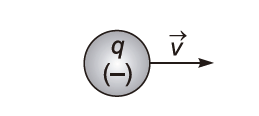
\includegraphics[width=0.8\linewidth]{img/carga moviendose.png}

        \small{\textbf{Figura 1.7.} Carga en movimiento.}
    \end{columns}
\end{frame}

% Diapositiva 2: Propiedades de la Energía Electromagnética
\begin{frame}
    \frametitle{Propiedades de la Energía Electromagnética}

    \textbf{Radiación Electromagnética:}
    \begin{itemize}
        \item Todos los cuerpos irradian energía electromagnética.
        \item La cantidad depende del movimiento de sus electrones.
    \end{itemize}

    \vspace{0.3cm}
    \textbf{Naturaleza Ondulatoria:}
    \begin{itemize}
        \item Se propaga en el espacio y en el tiempo con variaciones de intensidad.
    \end{itemize}

    \vspace{0.3cm}
    \textbf{Tipos de Energía Electromagnética:}
    \begin{itemize}
        \item Microondas, ondas de radio, rayos X, infrarrojos, ultravioleta.
        \item Luz visible (desde el rojo hasta el azul en el espectro).
    \end{itemize}

\end{frame}

\begin{frame}{Ondas electromagnéticas}
    \begin{figure}
        \centering
        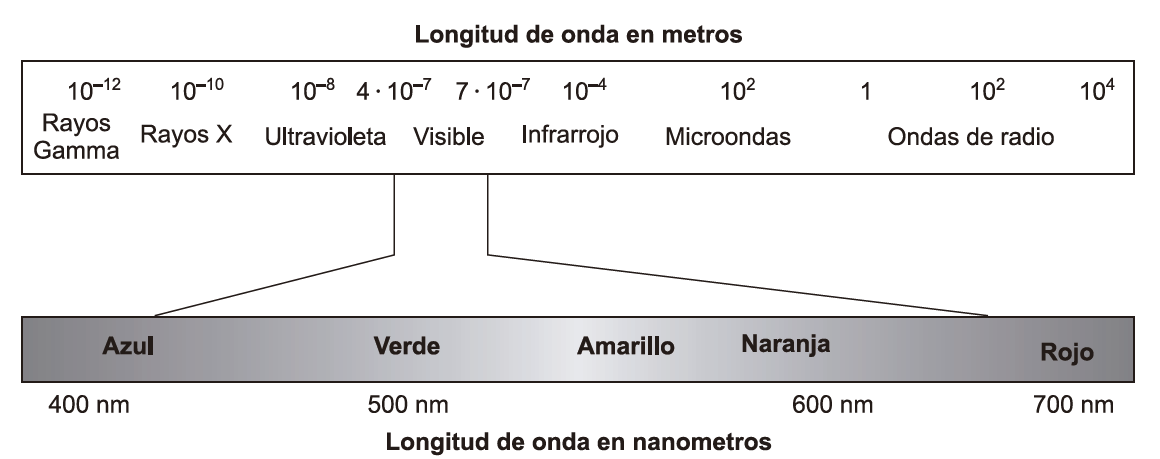
\includegraphics[width=1\linewidth]{img/ondas electromagneticas+.png}
        \caption{Ondas electromagneticas}
        %\label{fig:enter-label}
    \end{figure}
\end{frame}


% Diapositiva: Energía Nuclear y Tipos de Energía
\begin{frame}
    \frametitle{Energía Nuclear y Otras Manifestaciones de la Energía}

    \textbf{Energía Nuclear:}  
    Es la energía almacenada en los núcleos de los átomos, en el momento de su formación.  
    Mantiene unidos a los protones y neutrones mediante fuerzas nucleares fuertes y débiles.

    \centering
    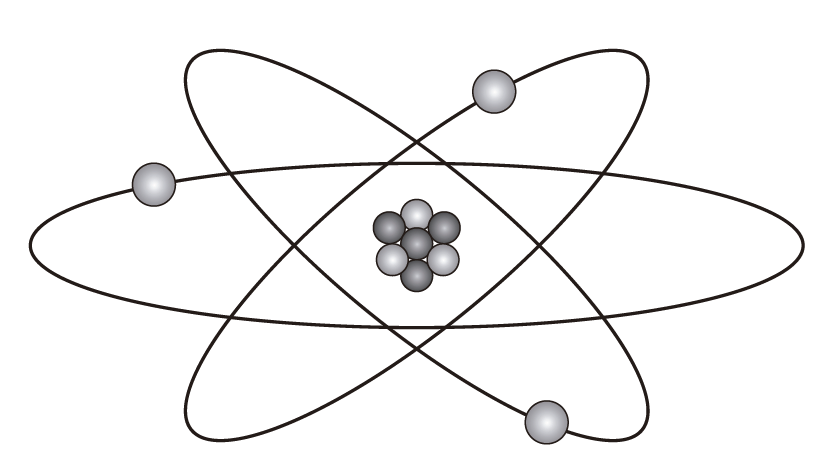
\includegraphics[width=0.4\linewidth]{img/atomo.png}

    \small{\textbf{Figura 1.9.} Representación de la energía nuclear.}

\end{frame}

% Diapositiva: Diversidad de Nombres en la Energía
\begin{frame}
    \frametitle{Diversidad de Nombres en la Energía}

    Aunque las formas fundamentales de la energía son cinco, en el lenguaje cotidiano se emplean diversos términos:
    
    \begin{itemize}
        \item \textbf{Energía potencial}: Energía almacenada en un cuerpo debido a su posición.
        \item \textbf{Energía térmica}: Energía asociada a la temperatura de un sistema.
        \item \textbf{Energía mecánica}: Suma de energía cinética y potencial de un cuerpo.
        \item \textbf{Energía eléctrica}: Movimiento de electrones en un conductor.
    \end{itemize}

    Sin embargo, algunos términos son incorrectos, ya que describen la forma de transmisión de la energía más que un tipo de energía en sí misma.

\end{frame}

% Diapositiva: Energía Eléctrica y Energía Térmica
\begin{frame}
    \frametitle{Energía Eléctrica y Energía Térmica}

    \textbf{Energía Eléctrica:}  
    \begin{itemize}
        \item Es el movimiento de electrones en un conductor.
        \item Se genera a partir de diferentes fuentes: generadores, pilas, termopares, etc.
        \item Se transforma en energía electromagnética, térmica o mecánica.
    \end{itemize}

    \vspace{0.3cm}
    \textbf{Energía Térmica:}  
    \begin{itemize}
        \item No es un tipo de energía en sí, sino un \textbf{flujo de energía térmica}.
        \item Se transfiere de un cuerpo más caliente a otro más frío.
        \item Similar a la lluvia: el calor no se almacena, sino que se transfiere.
    \end{itemize}

\end{frame}

% Diapositiva 1: Transformaciones Energéticas
\begin{frame}
    \frametitle{Transformaciones Energéticas y Rendimiento}

    \textbf{Definición:}  
    La energía permite realizar transformaciones en la materia a diferentes niveles:
    \begin{itemize}
        \item \textbf{Atómico:} En el núcleo o electrones de los átomos.
        \item \textbf{Molecular:} Mediante reacciones químicas.
        \item \textbf{Físico:} Cambios de estado de agregación.
    \end{itemize}

    \vspace{0.3cm}
    \textbf{Principio de Conservación:}
    \begin{itemize}
        \item La materia y la energía se conservan en todos los procesos.
        \item \textbf{Primera Ley de la Termodinámica:} ``La energía ni se crea ni se destruye, solo se transforma.''
    \end{itemize}

\end{frame}

% Diapositiva 2: Reacciones Químicas y Transformaciones Energéticas
\begin{frame}
    \frametitle{Reacciones Químicas y Transformaciones Energéticas}

    \textbf{Ejemplo: Reacciones Químicas}
    \begin{itemize}
        \item Los reactivos (\textbf{masa inicial}) se transforman en productos (\textbf{masa final}).
        \item La diferencia de energía entre ellos se intercambia con el medio.
    \end{itemize}

    \vspace{0.3cm}
    \textbf{Tipos de Reacciones:}
    \begin{itemize}
        \item \textbf{Exotérmicas:} Liberan energía al medio en forma de calor.
        \item \textbf{Endotérmicas:} Absorben energía del medio para llevarse a cabo.
    \end{itemize}

    \centering
    \fbox{
        \( 2C_4H_{10} + 13O_2 \rightarrow 8CO_2 + 10H_2O \)
    }

    \vspace{0.3cm}
    \textbf{Ejemplo:} Combustión del butano, una reacción fuertemente exotérmica.
\end{frame}

% Diapositiva 3: Transferencia de Energía y Reversibilidad
\begin{frame}
    \frametitle{Transferencia de Energía y Reversibilidad}

    \textbf{Energía Térmica Transferida:}
    \begin{itemize}
        \item Se manifiesta en forma de vibración de partículas (ejemplo: CO$_2$ y H$_2$O en la combustión).
        \item También se emite como energía electromagnética (luz visible e infrarroja).
    \end{itemize}

    \vspace{0.3cm}
    \textbf{Irreversibilidad en la Transferencia de Energía:}
    \begin{itemize}
        \item La energía térmica pasa de cuerpos con temperatura alta a otros con temperatura menor.
        \item Este proceso no es reversible (segunda ley de la termodinámica).
    \end{itemize}

\end{frame}

% Diapositiva 4: Equilibrio Térmico
\begin{frame}
    \frametitle{Equilibrio Térmico}

    \textbf{Ejemplo: Transferencia de Energía entre dos Cuerpos}
    \begin{itemize}
        \item Dos cuerpos en contacto intercambian energía térmica.
        \item La temperatura se equilibra cuando $T_1 = T_2$.
        \item No es posible que el cuerpo más frío transfiera energía al más caliente sin un aporte externo.
    \end{itemize}

    \centering
    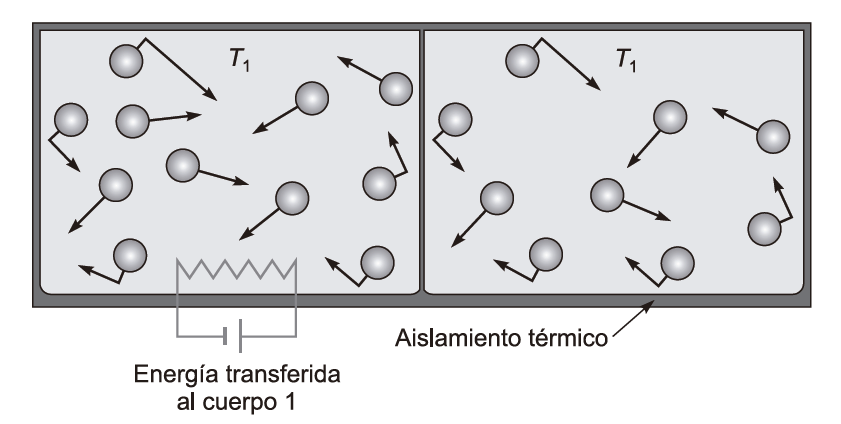
\includegraphics[width=0.5\linewidth]{img/equilibrio_termico.png}

    \small{\textbf{Figura 1.10.} Representación del equilibrio térmico.}

\end{frame}


% Diapositiva 1: Intercambios Energéticos
\begin{frame}
    \frametitle{Intercambios Energéticos}
    \textbf{Ejemplo: Elevación de una Masa}
    \small
    \begin{itemize}
        \item La energía se transfiere desde el Sol hasta el trabajo físico realizado por una persona.
        \item La energía del Sol es absorbida por las plantas mediante la fotosíntesis.
        \item Al ingerir alimentos vegetales, la energía química se almacena en los músculos.
        \item Esta energía química se convierte en energía mecánica al levantar la masa de 50 kg a 10 m.
    \end{itemize}

    \centering
    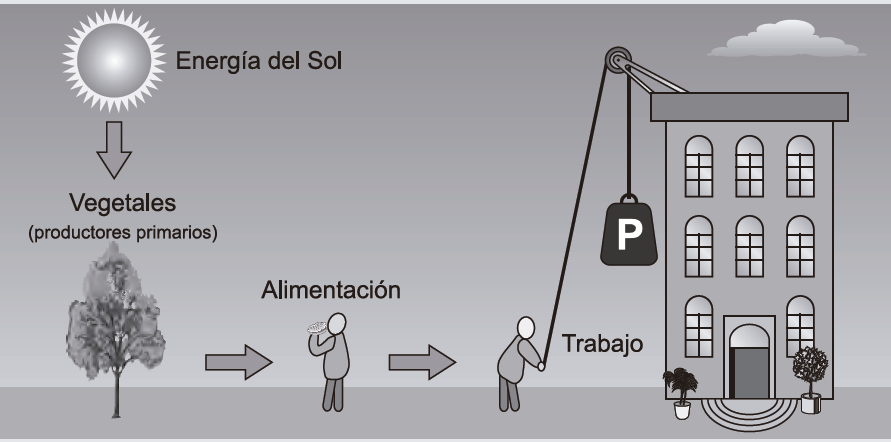
\includegraphics[width=0.45\linewidth]{img/intercambios_energeticos.png}

 %   \small{\textbf{Figura 1.11.} Intercambios energéticos.}
\end{frame}

% Diapositiva 2: Balance Energético
\begin{frame}
    \frametitle{Balance Energético del Proceso}
\small
    \textbf{Transferencias Energéticas}
    \begin{itemize}
        \item La energía fluye a través de distintas etapas: Sol → Planta → Persona → Trabajo.
        \item Se intercambia entre los sistemas en forma de energía térmica, química y mecánica.
    \end{itemize}

    %\vspace{0.1cm}
    \textbf{Balance Energético}
    \begin{itemize}
        \item La suma de la energía inicial del Sol es igual a la energía final almacenada en los distintos sistemas.
        \item La energía no se pierde, solo se transforma en diferentes manifestaciones.
    \end{itemize}

    \centering
    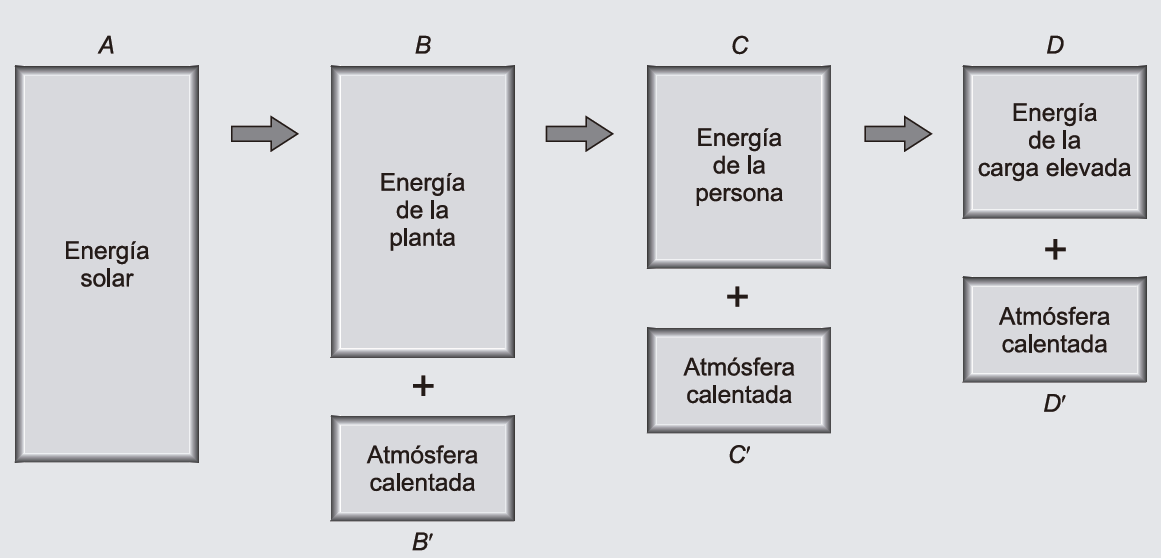
\includegraphics[width=0.4\linewidth]{img/tranferencias_energeticas.png}

   % \small{\textbf{Figura 1.12.} Transferencias energéticas.}
\end{frame}

% Diapositiva 3: Rendimiento de un Proceso Energético
\begin{frame}
    \frametitle{Rendimiento Energético}

    \begin{columns}
        % Columna izquierda con el texto
        \column{0.65\textwidth}
        \textbf{Concepto de Eficiencia Energética:}
        \begin{itemize}
            \item Es la relación entre la energía útil obtenida y la energía inicial suministrada.
            \item En motores eléctricos, el 90\% de la energía eléctrica se convierte en energía mecánica.
            \item En motores de combustión, solo el 20\% de la energía del combustible se transforma en trabajo útil.
        \end{itemize}

        \vspace{0.3cm}
        \textbf{Ejemplo: Motor de Gasolina}
        \begin{itemize}
            \item La gasolina tiene un contenido energético de 100 unidades.
            \item Solo 20 unidades se convierten en trabajo mecánico.
            \item El 80\% de la energía se disipa en forma de calor.
        \end{itemize}

        % Columna derecha con la imagen
        \column{0.35\textwidth}
        \centering
        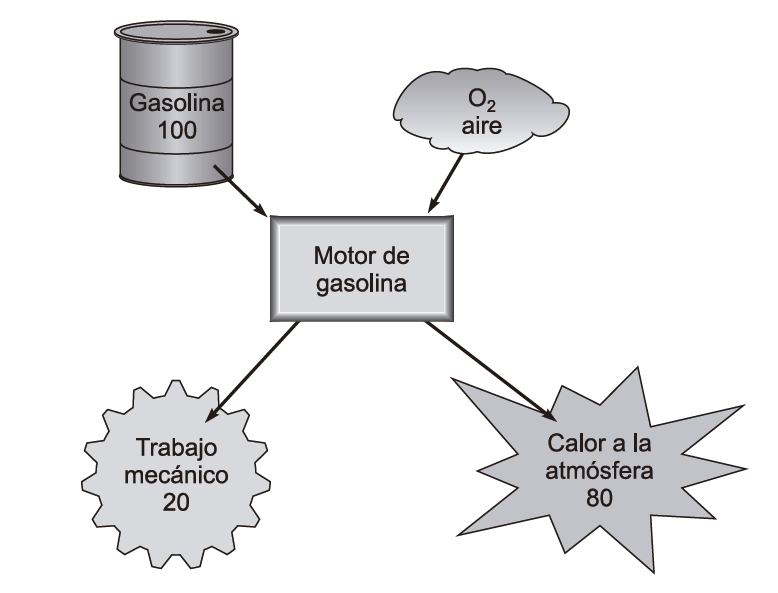
\includegraphics[width=\linewidth]{img/rendimiento_energetico.png}

        \small{\textbf{Figura 1.13.} Rendimiento de un proceso de cambio energético.}
    \end{columns}

\end{frame}


\begin{frame}[t] % Alinea el texto en la parte superior
    \frametitle{Energía Cinética Rotacional}

    La energía cinética también está asociada con el movimiento rotacional de los objetos en rotación.  
    La energía se expresa como:

    \[
    W = \frac{1}{2} I \omega^2
    \]

    donde $I$ es el momento de inercia del objeto y $\omega$ es su velocidad angular.  
   

    El momento de inercia se mide en unidades de kg$\cdot$m$^2$, y la velocidad angular en s$^{-1}$.  
    Como antes, la energía se mide en julios.  

    Los objetos que tienen tanto movimiento de traslación como de rotación poseen tanto energía cinética traslacional.
\end{frame}


\begin{frame}[t] % Alinea el texto en la parte superior
    \frametitle{Energía Térmica}
    \small
    La energía térmica de un gas resulta de la energía cinética del movimiento microscópico de sus moléculas.  Cada molécula de gas tiene una energía cinética asociada que se expresa como:

    \[
    \frac{1}{2} m v^2 = \frac{3}{2} k_B T = \frac{3}{2}nRT
    \]

    donde $m$ es la masa de la molécula, $v$ es su velocidad promedio, $k_B$ es la constante de Boltzmann  ($1.3806 \times 10^{-23}$ J/K) y $T$ es la temperatura absoluta en Kelvin.

    La energía interna total de un gas se obtiene multiplicando la ecuación anterior por el número de moléculas presentes.  
    Para trabajar con cantidades macroscópicas, se usa el número de moles $n$ y la constante de gas universal $R$, con:

   
    donde $R = N_A k_B = 8.315$ J/(mol·K) y $N_A$ es el número de Avogadro ($6.022 \times 10^{23}$ mol$^{-1}$).
\end{frame}

\begin{frame}
    \frametitle{Calor Específico y Calor Latente}

    En sólidos y líquidos, los cambios en la energía térmica se describen en términos del calor específico $C$.  
    Si se suministra una cantidad de energía $Q$ a un material de masa $m$, su temperatura aumentará en:

    \[
    \Delta T = \frac{Q}{m C}
    \]

    Los materiales con alto calor específico requieren más energía para aumentar su temperatura, 
    pero pueden almacenar grandes cantidades de energía térmica con pequeños cambios de temperatura.

    Cuando un sólido se calienta hasta su punto de fusión, se requiere energía adicional para fundirlo, conocida como \textbf{calor latente de fusión}.De manera similar, el \textbf{calor latente de vaporización} es la energía necesaria para que un líquido pase a gas sin cambiar su temperatura.
\end{frame}



\begin{frame}[t] % La opción [t] alinea el texto en la parte superior
    \frametitle{Ejemplo 1}
    
    Si un sistema produce 1 Btu de energía cada minuto, ¿cuál es la potencia producida en vatios?

    \pause % Hace que lo siguiente aparezca con un clic

    \textbf{Solución:}  
    \begin{itemize}
        \item 1 Btu = 1055 J
        \item Se libera en 60 s
    \end{itemize}

    La potencia se calcula como:

    \[
    P = \frac{E}{t} = \frac{1055 \text{ J}}{60 \text{ s}}
    \]

    \[
    P = 17.6 \text{ W}
    \]

\end{frame}
\begin{frame}[t] % La opción [t] alinea el texto en la parte superior
    \frametitle{Ejemplo 2}
    ¿Cuál es la energía cinética asociada con un automóvil de 1500 kg que viaja a 100 km/h?

    \pause % Pausa para mostrar la solución al hacer clic

    \textbf{Solución:} \\
    La velocidad convertida a m/s es: \\
    \[
    (100 \, \text{km/h}) \times \left(\frac{1000 \, \text{m/km}}{3600 \, \text{s/h}}\right) = 27.8 \, \text{m/s}
    \]
    Usando la ecuación de energía cinética: \\
    \[
    E = \frac{1}{2} m v^2 = (0.5) \times (1500 \, \text{kg}) \times (27.8 \, \text{m/s})^2 = 5.8 \times 10^5 \, \text{J}
    \]
\end{frame}

\begin{frame}[t] % La opción [t] alinea el texto en la parte superior
    \frametitle{Ejemplo 3}
    Una rueda en forma de un disco sólido con una masa de $m = 400$ kg, un diámetro de $d = 0.85$ m y un momento de inercia de $I = \frac{md^2}{8} = \frac{mr^2}{2}$ rueda sin deslizamiento. La velocidad de su centro de masa es de 30 m/s. Esta es una aproximación de una rueda en un tren de carga.

    Compare la energía cinética de traslación de la rueda con su energía rotacional.

    \pause % Pausa para mostrar la solución al hacer clic

    \textbf{Solución:} \\
    \textbf{Energía cinética de traslación:} \\
    \[
    E_{\text{traslación}} = \frac{1}{2} m v^2 = (0.5) \times (400 \, \text{kg}) \times (30 \, \text{m/s})^2 = 1.8 \times 10^5 \, \text{J}
    \]
\end{frame}
\begin{frame}{continuación}
     \textbf{Energía rotacional:} \\
    Si la rueda rueda sin deslizamiento, su velocidad angular es $\omega = \frac{v}{r}$. Sustituyendo en la ecuación de energía rotacional: \\
    \[
    E_{\text{rotacional}} = \frac{1}{2} I \omega^2 = \frac{1}{2} \left(\frac{m r^2}{2}\right) \left(\frac{v}{r}\right)^2 = \frac{1}{4} m v^2
    \]
     \textbf{Sustituyendo los valores:} \\
    \pause % Pausa para mostrar la sustitución
    \[
    E_{\text{rotacional}} = \frac{1}{4} m v^2 = (0.25) \times (400 \, \text{kg}) \times (30 \, \text{m/s})^2 = 9.0 \times 10^4 \, \text{J}
    \]


    \textbf{Comparación:} \\
    La energía rotacional es exactamente la mitad de la energía cinética de traslación. Esto es característico de un disco sólido que rueda sin deslizamiento.
\end{frame}

  



\begin{frame}[t] % La opción [t] alinea el texto en la parte superior
    \frametitle{Ejemplo 4}
    Una persona de 75 kg sube un tramo de escaleras con una altura vertical de 3 m. ¿Cuál es el cambio en la energía potencial de esa persona?

    \pause % Pausa para mostrar la solución al hacer clic

    \textbf{Solución:} \\
    El cambio en la energía potencial se calcula mediante la fórmula: \\
    \[
    \Delta E_{\text{potencial}} = m \cdot g \cdot h
    \]
    Donde:
    \begin{itemize}
        \item \( m = 75 \, \text{kg} \) (masa de la persona),
        \item \( g = 9.8 \, \text{m/s}^2 \) (aceleración debido a la gravedad),
        \item \( h = 3 \, \text{m} \) (altura vertical).
    \end{itemize}
\end{frame}

\begin{frame}{continuación}
     Sustituyendo los valores: \\
    \[
    \Delta E_{\text{potencial}} = (75 \, \text{kg}) \times (9.8 \, \text{m/s}^2) \times (3 \, \text{m}) = 2205 \, \text{J}
    \]
    \[
    \Delta E_{\text{potencial}} \approx 2.2 \times 10^3 \, \text{J}
    \]

\end{frame}
   

\begin{frame}[t] % Alinea el contenido en la parte superior
    \frametitle{Cálculo de Energía Térmica}

    \textbf{Ejemplo 5}  
    La capacidad calorífica específica del agua es de $4180$ J/(kg·°C).  
    Calcule la energía requerida para calentar $500$ g de agua desde $20^\circ$C hasta $80^\circ$C.

    \vspace{0.2cm}
    La ecuación para el calor transferido es:

    \[
    Q = m C \Delta T
    \]
 \pause % Pausa antes de mostrar la solución
    donde:
    \begin{itemize}
        \item $m = 0.500$ kg (masa del agua)
        \item $C = 4180$ J/(kg·°C) (calor específico)
        \item $\Delta T = 80^\circ \text{C} - 20^\circ \text{C} = 60^\circ \text{C}$ (cambio de temperatura)
    \end{itemize}
\end{frame}

\begin{frame}{Frame Title}
     Sustituyendo los valores:

    \[
    Q = (0.500 \, \text{kg}) (4180 \, \text{J/(kg·°C)}) (60^\circ \text{C})= 1.25 \times 10^5 \text{ J}
    \]

\end{frame}
   


\begin{frame}
\frametitle{Ejemplo 6: Longitud de onda de la luz amarilla}
\framesubtitle{Estimación del número de longitudes de onda entre un monitor y un usuario}

\textbf{Problema:}\\
Estimar el número de longitudes de onda de la luz amarilla que abarcan la distancia entre un monitor de computadora y un usuario.

\pause % Simula el clic para revelar la solución

\textbf{Solución:}\\
\begin{itemize}
    \item La longitud de onda de la luz amarilla es aproximadamente \( \lambda = 600 \, \text{nm} = 6.0 \times 10^{-7} \, \text{m} \).
    \item La distancia típica entre un usuario y el monitor es \( d = 0.5 \, \text{m} \).
    \item El número de longitudes de onda que caben en esta distancia es:
    \[
    N = \frac{d}{\lambda} = \frac{0.5 \, \text{m}}{6.0 \times 10^{-7} \, \text{m}} = 8.3 \times 10^5 \, \text{longitudes de onda}
    \]
\end{itemize}



\textbf{Resultado:}\\
El número de longitudes de onda de luz amarilla que abarcan la distancia es \( 8.3 \times 10^5 \).

\end{frame}
%%%%%%%%%%%%%%%%%%%%%%%%%%%%%%%%%%%%%%%%%%%%%%%%%%%%%%%%%%%%%%%%%%
\section{La energía en el Universo}
\begin{frame}
\frametitle{Introducción}
\framesubtitle{Repaso de las Fuentes de Energía}
\begin{itemize}
    \item Se realiza un repaso amplio de las fuentes de energía en la Tierra y el Universo.
    \item Enfoque en las transformaciones de la energía solar, que es la base de la mayoría de las energías disponibles (fósiles y renovables).
    \item Presentación sistemática de cada fuente:
    \begin{itemize}
        \item Origen.
        \item Potencial energético.
        \item Formas de aprovechamiento.
        \item Producción y consumo mundial.
        \item Duración prevista.
    \end{itemize}
    \item Análisis de la situación energética mundial y el papel crucial de las energías renovables.
\end{itemize}
\end{frame}

% Diapositiva 1: Formas de energía en el Universo
\begin{frame}
\frametitle{Formas de Energía en el Cosmos}
\begin{itemize}
    \item \textbf{Energía gravitacional}: Atracción entre masas (astros)
    \item \textbf{Energía cinética}: Movimiento de astros y sistemas cósmicos
    \item \textbf{Energía eléctrica}: Energía química en combustibles (local en Tierra)
    \item \textbf{Energía electromagnética}: Radiación estelar (luz, rayos cósmicos)
    \item \textbf{Energía nuclear}: Asociada a la formación de materia (predominante)
\end{itemize}
\begin{center}
    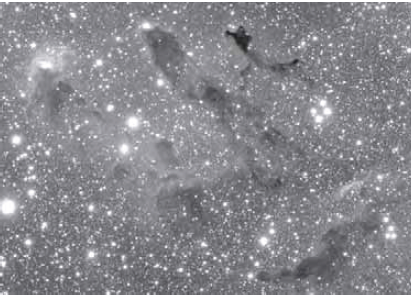
\includegraphics[width=0.3\textwidth]{img/cosmos.png} % Reemplazar con Figura 2.1
\end{center}
\end{frame}

% Diapositiva 2: Clasificación por entropía
\begin{frame}
\frametitle{Clasificación por Órdenes de Mérito}
\begin{enumerate}
    \item Energía gravitacional (menor entropía)
    \item Energía de movimiento (cinética)
    \item Energía nuclear
    \item Energía electromagnética
    \item Energía eléctrica/química (mayor entropía)
\end{enumerate}
\vspace{5mm}
\begin{block}{Principio de Degradación}
La energía superior puede transformarse en inferior, pero no al revés (excepto procesos locales en seres vivos con aumento global de entropía).
\end{block}
\end{frame}

% Diapositiva 3: Flujo energético y retardos cósmicos
\begin{frame}
\frametitle{Flujo de Energía y Retardos Cósmicos}
\begin{itemize}
    \item \textbf{Fuentes principales}: 
    \begin{itemize}
        \item Reacciones termonucleares estelares
        \item Contracción de masas (gravitación $\rightarrow$ cinética/electromagnética)
    \end{itemize}
    
    \item \textbf{¿Por qué persiste la energía gravitatoria?} 
    \begin{itemize}
        \item Baja densidad del Universo (tiempos de colapso $\sim$100 millones de años)
        \item Rotación de astros y galaxias (energía cinética estabilizadora)
        \item Combustión lenta de hidrógeno en estrellas
    \end{itemize}
\end{itemize}
\end{frame}

% Diapositiva 4: Fenómenos energéticos cósmicos
\begin{frame}
\frametitle{Fenómenos Energéticos Extremos}
\begin{columns}
\column{0.5\textwidth}
\begin{itemize}
    \item \textbf{Rayos cósmicos}: 
    \begin{itemize}
        \item Partículas ultraenergéticas
        \item Origen en supernovas/colapsos gravitatorios
    \end{itemize}
    
    \item \textbf{Radiogalaxias}: 
    \begin{itemize}
        \item Nubes de electrones energéticos
    \end{itemize}
\end{itemize}

\column{0.5\textwidth}
\begin{itemize}
    \item \textbf{Quásares y púlsares}: 
    \begin{itemize}
        \item Fuentes intensas de rayos X
        \item Objetos compactos en rápida rotación
    \end{itemize}
    
    \item \textbf{Supernovas}: 
    \begin{itemize}
        \item Explosiones termonucleares estelares
    \end{itemize}
\end{itemize}
\end{columns}
\begin{center}
    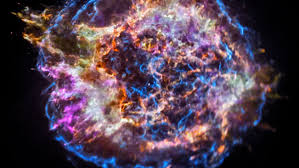
\includegraphics[width=0.4\textwidth]{img/supernova.jpg} % Reemplazar con imagen apropiada
\end{center}
\end{frame}

% Diapositiva 5: Retardos termonucleares
\begin{frame}
\frametitle{Mecanismos de Retardo Cósmico}
\begin{itemize}
    \item \textbf{Retardo termonuclear}: 
    \begin{itemize}
        \item Combustión lenta de H$_2$  (10$^{18}$ veces más lenta que deuterio/tritio)
        \item Evita colapso estelar inmediato
    \end{itemize}
    
    \item \textbf{Transporte lento de energía}: 
    \begin{itemize}
        \item Conducción térmica en núcleos planetarios/estelares
        \item Tiempos de enfriamiento de millones de años
    \end{itemize}
    
    \item \textbf{Incompresibilidad planetaria}: 
    \begin{itemize}
        \item Impide alcanzar condiciones para fusión nuclear
    \end{itemize}
\end{itemize}
\end{frame}

% Diapositiva 6: Conclusión
\begin{frame}
\frametitle{Conclusión}
\begin{itemize}
    \item El Universo mantiene un equilibrio dinámico mediante retardos en la degradación energética
    \item Los procesos cósmicos involucran transformaciones energéticas a escalas colosales
    \item Fenómenos extremos (supernovas, rayos cósmicos) son clave en el flujo energético
    \item La comprensión de estos mecanismos es esencial para la astrofísica moderna
\end{itemize}
\end{frame}

\section{Energia de la Tierra}
\begin{frame}{La energía de la Tierra Introducción}
    \begin{itemize}
        \item La energía de la Tierra fluye continuamente hacia dentro y fuera del planeta.
        \item Principales fuentes de energía:
        \begin{itemize}
            \item \textbf{Nuclear}: contenida en los núcleos de la materia y liberada en procesos de fisión y fusión.
            \item \textbf{Electromagnética}: procedente del Sol, vital para el clima y la fotosíntesis.
            \item \textbf{Gravitacional}: interacción Tierra-Luna-Sol, fundamental en las mareas.
        \end{itemize}
        \item La energía cinética terrestre proviene de su rotación y traslación en el espacio.
    \end{itemize}
\end{frame}

\begin{frame}{Movimientos y Energía Cinética}
    \begin{columns}
        \begin{column}{0.5\textwidth}
            \begin{itemize}
                \item La Tierra se mueve a más de 100 km/s en el espacio.
                \item Su movimiento genera energía debido a:
                \begin{itemize}
                    \item Traslación alrededor del Sol.
                    \item Movimiento del Sistema Solar en la galaxia.
                    \item Desplazamiento de la galaxia en el universo.
                \end{itemize}
                \item Estos movimientos afectan el clima y los ciclos de energía en la Tierra.
            \end{itemize}
        \end{column}
        \begin{column}{0.5\textwidth}
            \centering
            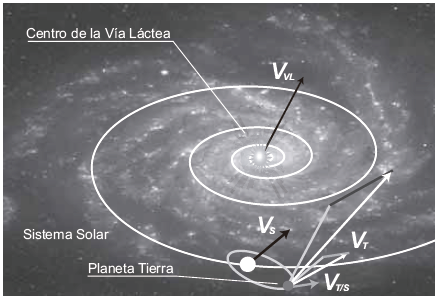
\includegraphics[width=0.9\textwidth]{img/movimienot_tierra.png}
            \footnotesize{Figura 2.3. Esquema de movimientos en el Sistema Solar.}
        \end{column}
    \end{columns}
\end{frame}

\begin{frame}{Fuentes Energéticas Disponibles}
    \begin{columns}
        \begin{column}{0.35\textwidth}
            \centering
            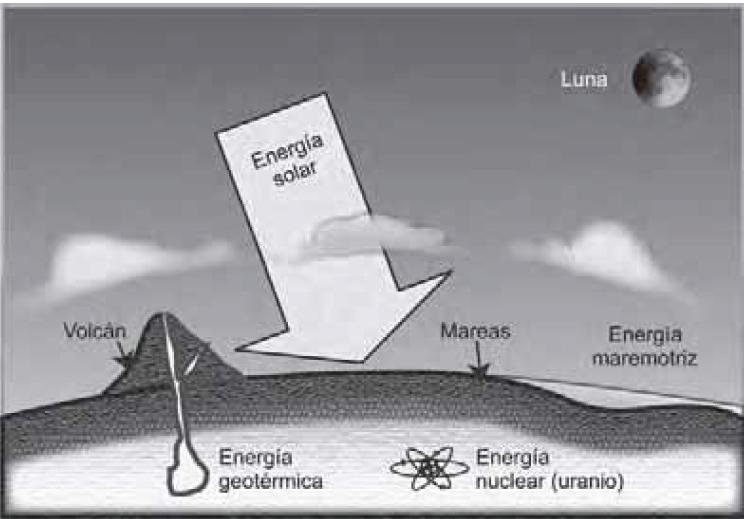
\includegraphics[width=1.2\textwidth]{img/fuentes_energeticas_tierra.png}
            \footnotesize{Figura 2.4. Fuentes energéticas de la Tierra.}
        \end{column}
        \begin{column}{0.65\textwidth}
            \begin{itemize}
                \item \textbf{Energía electromagnética}: Procedente del Sol, impulsa la fotosíntesis y regula la temperatura.
                \item \textbf{Energía nuclear}: Liberada en procesos de fisión (reactores nucleares) y fusión (en el Sol).
                \item \textbf{Energía gravitacional}: Su efecto en las mareas permite la generación de energía mareomotriz.
                \item \textbf{Energía geotérmica}: Generada por el calor interno de la Tierra, utilizada en energía geotérmica.
                \item \textbf{Energía química}: Almacenada en combustibles fósiles formados por restos orgánicos.
            \end{itemize}
        \end{column}
    \end{columns}
\end{frame}

\begin{frame}{Almacenamiento de Energía Solar}
    \begin{columns}
        \begin{column}{0.6\textwidth}
            \begin{itemize}
                \item Las hojas verdes captan radiación solar mediante fotosíntesis.
                \item La energía se almacena químicamente en biomasa y combustibles fósiles.
                \item Diferentes formas de almacenamiento:
                \begin{itemize}
                    \item Biomasa: madera, residuos agrícolas, biogás.
                    \item Combustibles fósiles: carbón, petróleo, gas natural, pizarras bituminosas y arenas asfálticas.
                    \item Energía térmica en los océanos y en la atmósfera.
                \end{itemize}
                \item La energía almacenada es clave para la sostenibilidad y el desarrollo tecnológico.
            \end{itemize}
        \end{column}
        \begin{column}{0.4\textwidth}
            \centering
            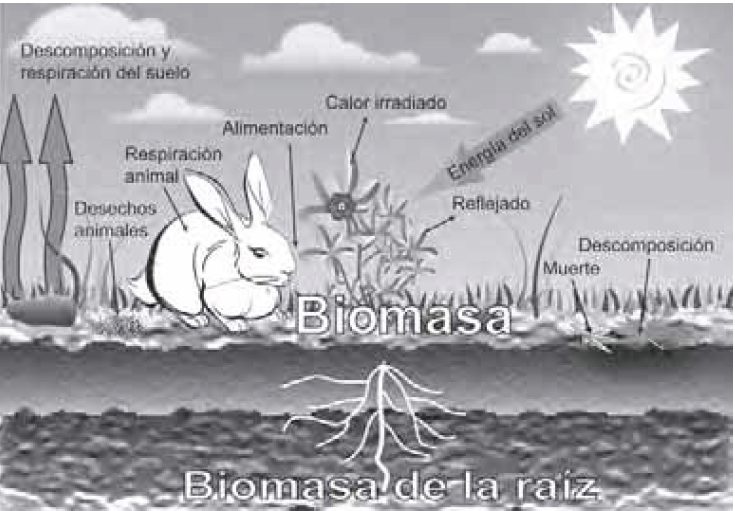
\includegraphics[width=1\textwidth]{img/almacenamienot_Energia.png}
            \footnotesize{Figura 2.5. Almacenamiento de energía solar mediante fotosíntesis.}
        \end{column}
    \end{columns}
\end{frame}

\begin{frame}{Distribución de la energía solar incidente}
    \begin{itemize}
        \item Energía solar total recibida en la atmósfera superior: aprox.\ 174\,PW $\approx$ 5\,489\,040\,TWh/año.
        \item Energía reflejada al espacio (~35\,\%): $\approx$ 1\,921\,164\,TWh/año.
        \item Energía absorbida (~65\,\%): $\approx$ 3\,567\,876\,TWh/año.
        \begin{itemize}
            \item Absorbida por la superficie terrestre (suelo y océanos): $\approx$ 2\,500\,000\,TWh/año.
            \item Absorbida directamente por la atmósfera: $\approx$ 1\,067\,876\,TWh/año.
        \end{itemize}
        \item Dentro del flujo absorbido por la superficie:
        \begin{itemize}
            \item Evaporación (calor latente $\rightarrow$ ciclo hidrológico): $\approx$ 19\,\% del total $\approx$ 1\,043\,000\,TWh/año.
            \item Convección y turbulencia (viento): $\approx$ 9\,\% del total absorbido $\approx$ 494\,000\,TWh/año.
            \item Radiación térmica directa y absorbida por gases (incluye reemisión): flujo restante.
            \item Fotosíntesis: captura $\approx$ 140\,TW ($\approx$ 0{,}08\,\% del flujo incidente) $\approx$ 1\,226\,TWh/año.
        \end{itemize}
    \end{itemize}
\end{frame}




\begin{frame}{Diagrama de distribución de la energía}
    \centering
    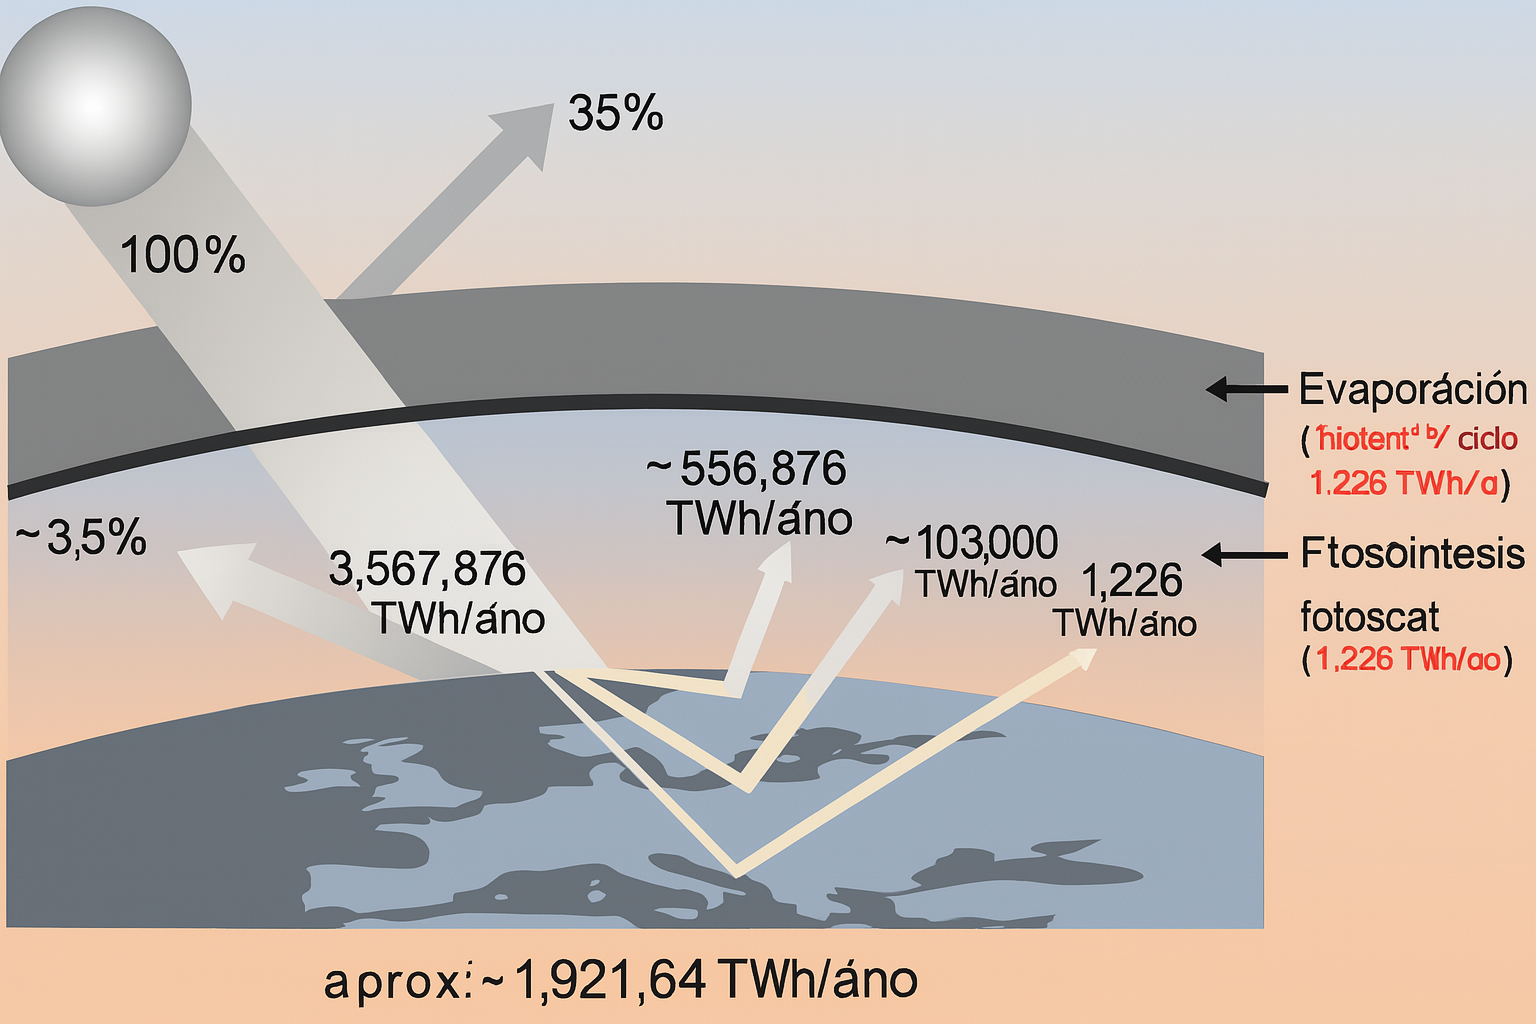
\includegraphics[width=0.7\textwidth]{img/distribucion_energia_solar.png}
    
    \footnotesize{Figura 2.6. Distribución de la energía solar incidente en la Tierra.}
\end{frame}
\begin{frame}{Clasificación de las fuentes energéticas}
    \begin{figure}
        \centering
        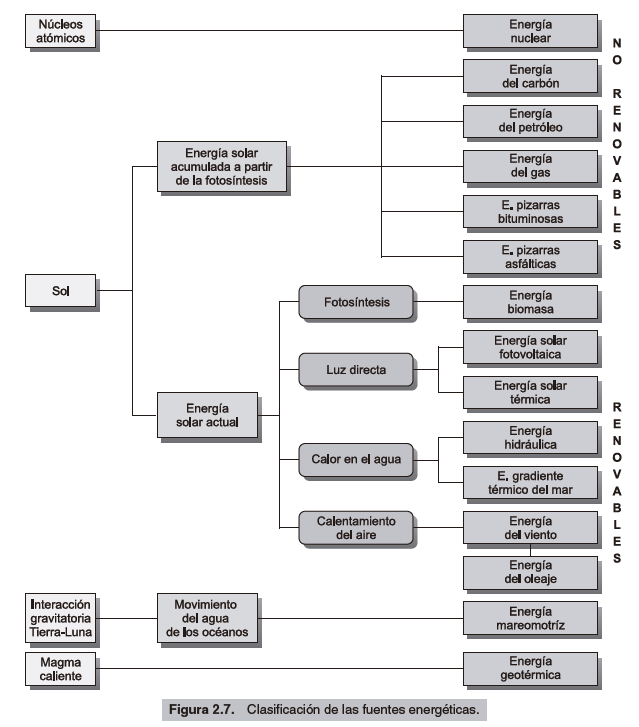
\includegraphics[width=0.5\linewidth, angle=90]{img/clasificacion de las fuentes.png}
        %\caption{Enter Caption}
        %\label{fig:enter-label}
    \end{figure}
\end{frame}

%\section{Consumo Global de Energía en la Tierra}
\begin{frame}{Consumo Global de Energía en la Tierra}
    \begin{itemize}
        \item Diferenciación entre recursos y reservas:
        \begin{itemize}
            \item \textbf{Recursos}: Cantidades totales conocidas o supuestas de una fuente energética.
            \item \textbf{Reservas}: Parte de los recursos que pueden ser explotadas con tecnología y costos actuales.
        \end{itemize}
        \item Clasificación de reservas:
        \begin{itemize}
            \item \textbf{Comprobadas}: Con información certera sobre su existencia y volumen.
            \item \textbf{No comprobadas}: Con estimaciones razonables basadas en estudios geológicos.
        \end{itemize}
        \item Un recurso puede convertirse en reserva si:
        \begin{itemize}
            \item Se mejoran las técnicas de extracción.
            \item Aumenta el precio de venta de la energía.
        \end{itemize}
    \end{itemize}
\end{frame}

\begin{frame}{Ciclo de Vida de un Recurso No Renovable}
    \begin{columns}
        \begin{column}{0.55\textwidth}
            \begin{itemize}
                \item La explotación de un recurso no renovable lleva inevitablemente a su agotamiento.
                \item La producción tiende a crecer exponencialmente al inicio.
                \item Posteriormente, el crecimiento se ralentiza y alcanza un pico.
                \item Finalmente, la producción disminuye progresivamente hasta su desaparición.
                \item Si se conocen las tasas de producción y las reservas, se puede estimar la vida útil de una fuente energética.
            \end{itemize}
        \end{column}
        \begin{column}{0.45\textwidth}
            \centering
            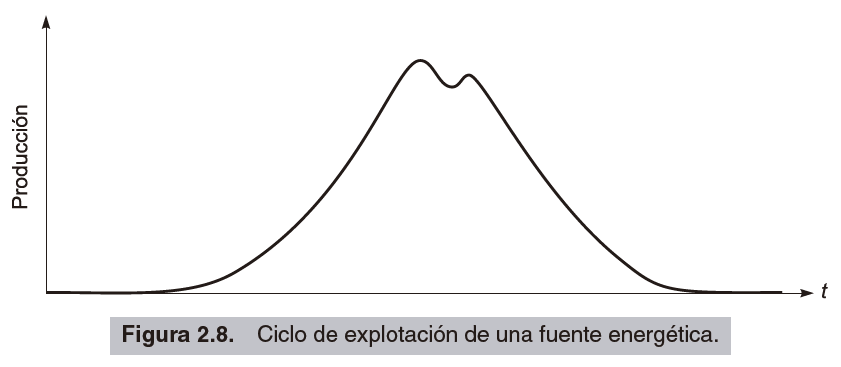
\includegraphics[width=0.9\textwidth]{img/ciclo explotacion.png}
            \footnotesize{Figura 2.8. Ciclo de explotación de una fuente energética.}
        \end{column}
    \end{columns}
\end{frame}

\begin{frame}{Consumo Total de Energía Primaria (2024)}
    \begin{itemize}
        \item Consumo total mundial: \textbf{15166 millones de Tep} (≈ 636 EJ ≈ 176 737 TWh)
        \item \textbf{Fuentes principales:}
        \begin{itemize}
            \item Petróleo: \textbf{52292 TWh} (29-31\%)
            \item Gas natural: \textbf{41278 TWh} (23\%)
            \item Carbón: \textbf{45 850 TWh} (26-28\%)
            \item Nuclear: \textbf{6872 TWh} (4-5\%)
            \item Hidráulica: \textbf{10 861 TWh} (14-15\%)
            \item Renovables modernas (solar, eólica, bioenergía, otras): \textbf{25 980 TWh} (≈ 14-15\%)
        \end{itemize}
    \end{itemize}
  Datos obtenidos de Our World in Data y Energy Institute (Statistical Review 2024)%
    \footnote{\url{https://ourworldindata.org/energy}, consultado el 20 de Enero de 2025}.
\end{frame}

\begin{frame}{Consumo por Regiones (2024)}
    \begin{itemize}
        \item Consumo total mundial: \textbf{15166 millones de Tep}
        \item \textbf{Distribución regional:}
        \begin{itemize}
            \item Asia : \textbf{841.87 millones de Tep} (5{,}55\%)
            \item América del Norte: \textbf{290.5 millones de Tep} (1{,}92\%)
            \item Europa y Eurasia: \textbf{334.1 millones de Tep} (2{,}2\%)
            \item Colombia: \textbf{52.9  millones de Tep} (0{,}348\%)
        \end{itemize}
    \end{itemize}
    Datos obtenidos de Our World in Data y Energy Institute (Statistical Review 2024)%
    \footnote{\url{https://ourworldindata.org/energy}, consultado el 27 de agosto de 2025}.
\end{frame}


\begin{frame}{Consumo de Energía Primaria por País (2024)}
    \begin{itemize}
        \item Consumo mundial total: \textbf{15166 millones de Tep}
        \item \textbf{Principales países:}
        \begin{itemize}
            \item China: \textbf{4212.4 millones de Tep} (27{,8\%})
            \item Estados Unidos: \textbf{2281 millones de Tep} (15{,1\%})
            \item India: \textbf{975,1 millones de Tep} (6{,4\%})
            \item Rusia: \textbf{778 millones de Tep} (5{,1\%})
            \item Japón: \textbf{411 millones de Tep} (2{,7\%})
            \item Alemania: \textbf{275 millones de Tep} (1{,8\%})
            \item Colombia: \textbf{52.9 millones de Tep} (0{,34\%})
        \end{itemize}
    \end{itemize}
    Los datos utilizados en este trabajo fueron obtenidos de la plataforma \textit{Our World in Data}%
    \footnote{\url{https://ourworldindata.org/energy}, consultado el 27 de agosto de 2025}.
\end{frame}





\begin{frame}{Biomasa y su Impacto (2025)}
    \begin{itemize}
        \item Más de \textbf{2\,000 millones de personas} (~25\,\% de la población mundial) aún dependen de biomasa tradicional (madera, residuos orgánicos) para cocinar y calefacción.
        \item Esta práctica genera \textbf{contaminación doméstica} severa, causando hasta \textbf{4 millones de muertes al año} por enfermedades respiratorias.
        \item El uso insostenible de biomasa está vinculado a la \textbf{deforestación acelerada}, especialmente en África (90\,\% de la población depende de leña) y al aumento de emisiones de CO₂.
        \item La \textbf{biomasa moderna} (computada en estadísticas) representa el 55\,\% de las renovables y aporta más del 6\,\% al suministro energético global.
        \item Crece la preocupación: países como Corea del Sur están reduciendo subsidios por el impacto en selvas importadas para pellets de madera.
    \end{itemize}
\end{frame}




\section{Energía Nuclear de Fisión}
\begin{frame}{Origen de la Energía Nuclear de Fisión}
    \begin{itemize}
        \item La energía de fisión se basa en la ruptura del núcleo de elementos pesados como el \textbf{uranio (U)}, \textbf{torio (Th)} y \textbf{plutonio (Pu)}, mediante bombardeo con neutrones lentos.
        \item El \textbf{uranio}, símbolo \textbf{U} y número atómico \textbf{92}, es el único elemento presente en la naturaleza que se utiliza directamente como material fisionable en reactores nucleares.
        \item Su isótopo más abundante es el \textbf{U-238}, aunque el más utilizado en reactores es el \textbf{U-235}, que representa solo el \textbf{0{,}7\,\%} del uranio natural.
        \item Se encuentra en más de \textbf{100 minerales}, destacando la \textbf{uraninita} (también llamada \textit{pechblenda}) y la \textbf{carnotita}.
        \item Para que la extracción sea rentable, el contenido de uranio en el mineral debe superar las \textbf{1\,000 ppm} (partes por millón).
    \end{itemize}
\end{frame}


\begin{frame}{Reacción Nuclear de Fisión}
    \begin{itemize}
        \item Cuando el núcleo de un átomo de \textbf{U-235} (uranio-235) es alcanzado por un neutrón (lento o rápido), se divide en dos núcleos más ligeros: \textbf{Bario-142} y \textbf{Kriptón-91}, que se desplazan a gran velocidad.
        \item En el proceso se liberan \textbf{dos o más neutrones} y una intensa \textbf{radiación gamma} ($\gamma$).
        \item La reacción que ocurre es:
        \[
        {}^{235}_{92}\text{U} + {}^1_\text{n} \rightarrow {}^{142}_{56}\text{Ba} + {}^{91}_{36}\text{Kr} + ^1_\text{n} + \text{210 MeV}
        \]
        \item La energía (~210 MeV) proviene de la diferencia de masa entre el núcleo original y la suma de las masas de los productos, según la ecuación de Einstein $E = \Delta m c^2$.
        \small
        \item La \textbf{reacción en cadena} se mantiene si se alcanza una \textbf{masa crítica} y se utilizan \textbf{moderadores} (agua ligera o pesada) para ralentizar los neutrones.
        \item Las \textbf{barras de control} (de boro o cadmio) absorben neutrones y regulan la potencia de la reacción.
    \end{itemize}
\end{frame}


\begin{frame}{Potencial Energético del Uranio-235}
    \begin{itemize}
        \item \textbf{1 tonelada de U-235 completamente fisionado} libera aproximadamente \textbf{8\,000\,000 MWh} (8 TWh).
        \item Esto equivale a:
        \begin{itemize}
            \item \textbf{~10\,000 toneladas de petróleo crudo}.
            \item \textbf{~14\,000 toneladas de carbón}.
        \end{itemize}
        \item Para generar \textbf{1 GWh} de energía eléctrica neta, una central nuclear requiere:
        \begin{itemize}
            \item Aproximadamente \textbf{25 a 30 kg de U-235 fisionable efectivo}.
            \item Lo que equivale a \textbf{1 tonelada de uranio natural} con un enriquecimiento promedio del 3–5 \%.
        \end{itemize}
        \item La energía de fisión de U-235 es más de \textbf{1 millón de veces mayor} que la energía por unidad de masa de combustibles fósiles.
    \end{itemize}
    \vspace{0.5em}
    \small{Datos actualizados con base en IAEA, WNA y U.S. DOE (2023–2025).}
\end{frame}

\begin{frame}{Formas de Aprovechamiento de la Energía Nuclear}
    \begin{itemize}
        \item La energía liberada por fisión nuclear se manifiesta principalmente como \textbf{energía térmica}.
        \item Esta energía se utiliza para \textbf{calentar un fluido de trabajo} (comúnmente agua, pero también CO\textsubscript{2} supercrítico o sodio líquido en reactores avanzados).
        \item El fluido caliente se convierte en \textbf{vapor o gas a alta presión}, el cual impulsa una \textbf{turbina de vapor}.
        \item La turbina acciona un \textbf{generador eléctrico}, transformando la energía térmica en \textbf{energía mecánica} y luego en \textbf{electricidad}.
        \item Este proceso es similar al de una central térmica convencional, pero la fuente de calor es nuclear, no fósil.
    \end{itemize}
    \vspace{0.5em}
    \small{Actualizado con base en tecnologías de fisión empleadas hasta 2025, incluyendo reactores de Generación III+ y IV.}
\end{frame}


\begin{frame}{Reservas de Uranio Natural (Principales países, 2023–2025)}
    \begin{itemize}
        \item Australia: \textbf{3\,600\,000 tU} (~29\,\%)
        \item Kazajistán: \textbf{2\,900\,000 tU} (~23\,\%)
        \item Canadá: \textbf{1\,700\,000 tU} (~14\,\%)
        \item Rusia: \textbf{1\,200\,000 tU} (~10\,\%)
        \item Namibia: \textbf{1\,000\,000 tU} (~8\,\%)
        \item EE.UU.: \textbf{180\,000 tU} (~1{,}4\,\%)
        \item Mongolia: \textbf{350\,000 tU} (~3\,\%)
    \end{itemize}
    \vspace{0.5em}
    \small{Fuente: NEA/IAEA “Red Book” 2023, consultado en julio de 2025.}
\end{frame}

\begin{frame}{Consumo de Uranio en Centrales Nucleares}
    \textbf{Consumo global (2023):} aproximadamente \textbf{67\,500 tU/año}  
    (equivalentes a ≈ \textbf{785\,000 TJ} ≈ \textbf{74 millones TWh-eq primarios})  
    \vspace{0.5em}
    \begin{itemize}
        \item Estados Unidos: ≈ \textbf{19\,000 tU} (~28\,\% del total)
        \item China: ≈ \textbf{9\,300 tU} (~14\,\%)
        \item Francia: ≈ \textbf{7\,500 tU} (~11\,\%)
        \item Rusia: ≈ \textbf{6\,000 tU} (~9\,\%)
        \item Corea del Sur: ≈ \textbf{5\,000 tU} (~7\,\%)
        \item Japón: ≈ \textbf{4\,000 tU} (~6\,\%)
        \item España: ≈ \textbf{1\,200 tU} (~2\,\%)
    \end{itemize}
    \vspace{0.5em}
    \small{Fuente: World Nuclear Association – “Supply of Uranium” (2024) y NEA/IAEA “Red Book” (2023–2025); consumo estimado por país según generación nuclear de electricidad 2023.}
\end{frame}


\begin{frame}{Duración Prevista de las Reservas de Uranio}
    \begin{itemize}
        \item Según el \textit{Red Book} (NEA/IAEA 2023), con el ritmo actual de consumo (~67\,500 tU/año):
        \begin{itemize}
            \item Las \textbf{reservas identificadas de bajo costo} (hasta 40 US\$/kgU) tienen una duración estimada de \textbf{~28 años}.
            \item Si se incluyen \textbf{todas las reservas recuperables a costos razonables} (hasta 130 US\$/kgU), la duración estimada es de aproximadamente \textbf{80–90 años}.
        \end{itemize}
        \item Estas proyecciones no consideran:
        \begin{itemize}
            \item Posibles descubrimientos futuros o recuperación de recursos no convencionales.
            \item Avances en reactores rápidos, reciclaje o torio.
        \end{itemize}
        \item El \textbf{60\,\%} de las reservas identificadas se concentran en solo 3 países: \textbf{Australia, Kazajistán y Canadá}.
    \end{itemize}
    \vspace{0.5em}
    \small{Fuente: OECD-NEA / IAEA “Uranium 2023: Resources, Production and Demand”, consultado en 2025.}
\end{frame}


\section{Energía Nuclear de Fusión}
\begin{frame}{Origen de la Energía Nuclear de Fusión}
    \small
    \begin{itemize}
        \item La \textbf{fusión nuclear} es el proceso en el que \textbf{dos núcleos ligeros}, típicamente \textbf{deuterio (D)} y \textbf{tritio (T)}, se combinan para formar un núcleo más pesado (helio), liberando una gran cantidad de energía.
        \item La diferencia de masa entre los núcleos iniciales y el núcleo final se convierte en energía de acuerdo con la ecuación de Einstein: $E = \Delta m c^2$.
        \item Para que ocurra la fusión, se debe \textbf{superar la repulsión electrostática} entre los núcleos, lo cual requiere condiciones extremas de \textbf{temperatura} (más de 100 millones °C) y \textbf{presión}.
        \item El \textbf{Sol y otras estrellas} funcionan como reactores de fusión natural, donde el hidrógeno se transforma en helio, liberando energía que sustenta su radiación.
        \item En la Tierra, proyectos como \textbf{ITER} y \textbf{NIF} están desarrollando reactores experimentales de confinamiento magnético (tokamak) e inercial, buscando lograr fusión controlada.
    \end{itemize}
\end{frame}


\begin{frame}{Reacciones de Fusión}
    \begin{itemize}
        \item En el \textbf{Sol}, la fusión ocurre mediante una serie de reacciones de la cadena protón-protón. De forma resumida:
        \[
        4\,{}^1\text{H} + 2e \rightarrow {}^4\text{He} + 2\,{}^1\text{n}+ + 2\nu_e + \gamma + 26{,}7\,\text{MeV}
        \]
        \item En la Tierra, la reacción más viable es la \textbf{deuterio-tritio (D-T)}:
        \[
        {}^2_1\text{H} + {}^3_1\text{H} \rightarrow {}^4_2\text{He} + {}^1_n + 17{,}6\,\text{MeV}
        \]
        \item El \textbf{deuterio (D)} es abundante en el agua de mar (≈ 30 g/m\textsuperscript{3}).
        \item El \textbf{tritio (T)} es radiactivo y escaso, pero puede generarse en el reactor mediante reacción con \textbf{litio}:
        \[
        {}^6_3\text{Li} + {}^1_n \rightarrow {}^4_2\text{He} + {}^3_1\text{H}
        \]
    \end{itemize}
\end{frame}


\begin{frame}{Potencial Energético de la Fusión}
    \begin{itemize}
        \item \textbf{1 m\textsuperscript{3}} de agua de mar contiene aproximadamente $10^{25}$ átomos de deuterio.
        \item Esa cantidad podría liberar una energía equivalente a \textbf{300 toneladas de carbón} o \textbf{1\,500 barriles de petróleo}.
        \item Se estima que \textbf{el 1\,\% del deuterio contenido en los océanos} podría generar hasta \textbf{500\,000 veces la energía total de todas las reservas fósiles conocidas}.
    \end{itemize}
\end{frame}


\begin{frame}{Formas de Aprovechamiento de la Fusión}
    \begin{itemize}
        \item Al igual que en la fisión, la energía térmica liberada en la fusión se utiliza para \textbf{calentar un fluido y generar vapor}, que a su vez acciona una \textbf{turbina de vapor} conectada a un generador eléctrico.
        \item \textbf{1 kg de helio} generado en la reacción de fusión libera una energía equivalente a la de \textbf{27\,000 toneladas de carbón}.
    \end{itemize}
\end{frame}


\begin{frame}{Reservas de Combustible para Fusión}
    \begin{itemize}
        \item El \textbf{deuterio} es prácticamente inagotable debido a su abundancia en el agua de mar (≈30 g/m\textsuperscript{3}).
        \item El \textbf{tritio}, aunque radiactivo y escaso de forma natural, puede ser producido de forma controlada mediante reacciones con \textbf{litio}, también abundante en la corteza terrestre y salmueras.
    \end{itemize}
\end{frame}


\begin{frame}{Consumo y Desarrollo Actual de la Fusión}
    \begin{itemize}
        \item Actualmente, \textbf{no existe generación eléctrica comercial por fusión nuclear}.
        \item El reactor experimental \textbf{ITER}, en construcción en Francia, está previsto que inicie operaciones de plasma en 2025 y pruebas completas hacia 2030.
        \item Proyectos como \textbf{NIF (EE.UU.)}, \textbf{JET (Reino Unido)} y \textbf{SPARC (MIT)} también avanzan en la validación de confinamiento inercial y magnético.
    \end{itemize}
\end{frame}


\begin{frame}{Duración de las Reservas de Fusión}
    \begin{itemize}
        \item La combinación de \textbf{deuterio abundante en el agua} y la capacidad de \textbf{producir tritio a partir del litio} hace que el combustible de fusión se considere \textbf{virtualmente inagotable} a escala humana.
        \item Esto convierte a la fusión en una de las fuentes energéticas más sostenibles a largo plazo.
    \end{itemize}
\end{frame}




\section{Energía del Carbón}
\begin{frame}{Energía del Carbón: Origen}
    El carbón se formó hace ~300 millones de años por la acumulación y enterramiento de grandes masas vegetales que, bajo condiciones anaeróbicas y alta presión, se transformaron de:
    \begin{itemize}
        \item Turba →
        \item Lignito →
        \item Carbón bituminoso →
        \item Antracita
    \end{itemize}
    Este proceso, denominado carbonización, se desarrolló durante el período Carbonífero (~359–299 Ma).
\end{frame}


\begin{frame}{Potencial Energético del Carbón}
    \begin{table}[]
        \centering
        \begin{tabular}{lcc}
            \hline
            \textbf{Tipo de carbón} & \textbf{Poder calorífico (kJ/kg)} & \textbf{(kWh/kg)} \\
            \hline
            Lignito & 17\,000–18\,000 & 5,0–5,0 \\
            Bituminoso & 24\,000–28\,000 & 6,7–7,8 \\
            Antracita & 30\,000–32\,000 & 8,3–8,9 \\
            \hline
        \end{tabular}
    \end{table}
    *Los rangos representan valores promedio globales actualizados.*
\end{frame}


\begin{frame}{Formas de Aprovechamiento del Carbón}
    \begin{itemize}
        \item Generación de calor para evaporar agua y producir energía mecánica en centrales térmicas.
        \item Industria siderúrgica, mediante coque derivado del carbón para fundir mineral de hierro.
        \item Conversión química por gasificación: obtención de combustibles líquidos y síntesis de productos químicos.
    \end{itemize}
\end{frame}

\begin{frame}{Reservas de Carbón (2024)}
    \begin{itemize}
        \item Reservas mundiales probadas: \textbf{1\,055 mil millones de toneladas} (Energy Institute, 2024)\footnote{\url{https://www.energyinst.org/statistical-review}}.
        \item Principales países: Estados Unidos, Rusia, China e India (≈ 76\,\% del total)\footnote{Fuente: Statistical Review of World Energy 2024}.
    \end{itemize}
\end{frame}



\begin{frame}{Producción y Consumo (2024)}
    \begin{itemize}
        \item Producción mundial: ≈ 8\,770 Mt (récord histórico)\footnote{IEA Coal 2024 Report}.
        \item China produce ~4\,053 Mt (47\,\% del total); India e Indonesia siguen como grandes productores\footnote{\url{https://www.iea.org/reports/coal-2024}}.
        \item Consumo global proyectado en 2025: ≈ 8\,700 Mt (~51\,\% en China)\footnote{Our World in Data, 2025}.
    \end{itemize}
\end{frame}




\begin{frame}{Duración Prevista de las Reservas}
    \begin{itemize}
        \item A ritmo actual (~8\,700 Mt/año), las reservas probadas durarían aproximadamente \textbf{121 años}\footnote{Cálculo propio con datos de Energy Institute, 2024}.
        \item Se estima que el consumo mundial alcanzará su \textit{“peak coal”} entre 2025 y 2027, con una posterior disminución por el avance de las energías renovables\footnote{IEA World Energy Outlook 2024}.
        \item La creciente demanda de \textbf{carbón metalúrgico} añade presión a ciertas reservas específicas, mientras que el \textbf{carbón térmico} es el más afectado por la transición energética.
    \end{itemize}
\end{frame}




\section{Energía del petroleo y del gas natural}
\begin{frame}{Origen del Petróleo y del Gas Natural}
    \small
    \begin{itemize}
        \item El \textbf{petróleo} se forma a partir de restos de organismos microscópicos (plancton y algas) depositados en fondos marinos, enterrados bajo sedimentos y sometidos a alta presión y temperatura durante millones de años.
        \item El \textbf{gas natural} puede originarse junto al petróleo (gas asociado) o por descomposición biológica en zonas pantanosas (biogás).
        \item Ambos son hidrocarburos: mezclas de compuestos orgánicos ricos en energía química.
    \end{itemize}
    \centering
    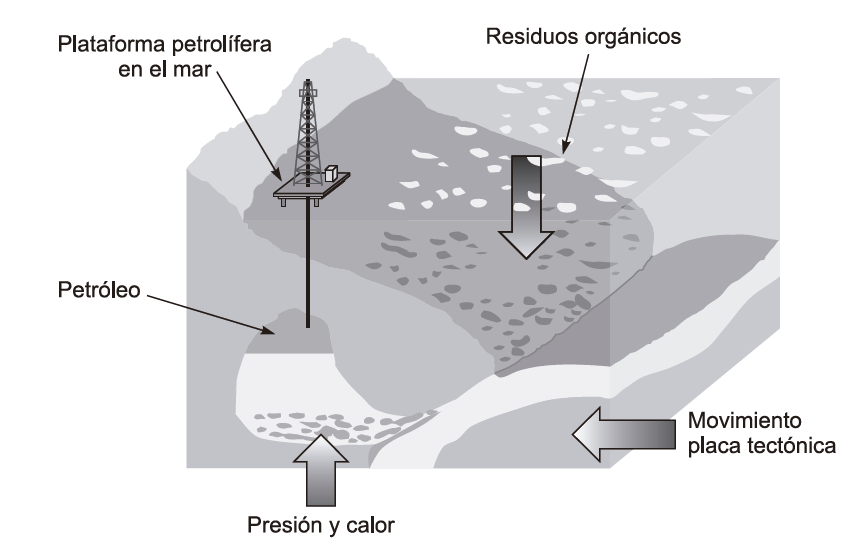
\includegraphics[width=0.4\textwidth]{img/Formacion_petroleo.png}
\end{frame}


\begin{frame}{Potencial Energético}
    \begin{itemize}
        \item \textbf{1 kg de petróleo} equivale aproximadamente a \textbf{11 kWh} o \textbf{39\,600 kJ}.
        \item \textbf{1 000 m\textsuperscript{3}} de gas natural equivale energéticamente a aproximadamente \textbf{900 kg de petróleo}.
        \item Ambos tienen una densidad energética alta, lo que los hace ideales como fuentes móviles de energía (transporte).
    \end{itemize}
\end{frame}


\begin{frame}{Formas de Aprovechamiento}
    \begin{itemize}
        \item \textbf{Petróleo:}
        \begin{itemize}
            \item Producción de combustibles líquidos: gasolina, diésel, queroseno, fuelóleo.
            \item Materia prima para la industria petroquímica: plásticos, fibras sintéticas, detergentes, fertilizantes, colorantes y medicamentos.
            \item Aplicaciones industriales: lubricantes, asfaltos, disolventes.
        \end{itemize}
        \item \textbf{Gas Natural:}
        \begin{itemize}
            \item Generación eléctrica en plantas térmicas y ciclos combinados (alta eficiencia).
            \item Uso doméstico: calefacción, cocción y agua caliente sanitaria.
            \item Combustible vehicular (GNV y GNL).
            \item Materia prima para la producción de hidrógeno (reformado con vapor) y fertilizantes (urea y amoníaco).
        \end{itemize}
    \end{itemize}
\end{frame}


\begin{frame}{Reservas de Petróleo (2024)}
    \begin{itemize}
        \item Reservas probadas: \textbf{1\,567 mil millones de barriles}\footnote{\url{https://www.energyinst.org/statistical-review}}.
        \item Principales países:
        \begin{itemize}
            \item Venezuela: \textbf{303 mil millones}
            \item Arabia Saudita: \textbf{267 mil millones}
            \item Irán: \textbf{209 mil millones}
            \item Canadá: \textbf{164 mil millones}
            \item \textbf{Colombia: 1,96 mil millones} (0,12\,\% del total mundial)
        \end{itemize}
    \end{itemize}
\end{frame}




\begin{frame}{Producción de Petróleo (2024)}
    \begin{itemize}
        \item Producción mundial: \textbf{≈ 101 millones de barriles/día}.
        \item Principales productores:
        \begin{itemize}
            \item Estados Unidos
            \item Arabia Saudita
            \item Rusia
            \item Canadá
        \end{itemize}
    \end{itemize}
\end{frame}


\begin{frame}{Reservas de Gas Natural (2024)}
    \begin{itemize}
        \item Reservas probadas: \textbf{≈ 208 billones de m\textsuperscript{3} (Tcm)}.
        \item Principales países:
        \begin{itemize}
            \item Rusia: ~47 Tcm
            \item Irán: ~34 Tcm
            \item Qatar: ~24 Tcm
            \item EE.UU.: ~19 Tcm
        \end{itemize}
    \end{itemize}
\end{frame}


\begin{frame}{Consumo Global (2024)}
    \begin{itemize}
        \item \textbf{Petróleo:} consumo mundial ≈ 100 millones de barriles/día.
        \item \textbf{Gas natural:} consumo global ≈ 4 000 millones de toneladas equivalentes/año.
        \item Principales consumidores: EE.UU., China, India y países de la UE.
    \end{itemize}
\end{frame}


\begin{frame}{Duración Estimada de las Reservas}
    \begin{itemize}
        \item Petróleo: \textbf{~47 años} de disponibilidad con consumo constante.
        \item Gas natural: \textbf{~52 años} de disponibilidad estimada.
        \item Factores que pueden alterar esta duración:
        \begin{itemize}
            \item Nuevas exploraciones y tecnologías de extracción.
            \item Aumento de la eficiencia energética y uso de fuentes renovables.
            \item Transición energética y descarbonización.
        \end{itemize}
    \end{itemize}
\end{frame}

\begin{frame}{Petróleo en Colombia (2024–2025)}
    \small
    \begin{itemize}
        \item \textbf{Reservas probadas:} \textbf{1,96 mil millones de barriles}  
        (≈ 7,5 años de autosuficiencia al ritmo actual)\footnote{\url{https://www.anh.gov.co/}}.

        \item \textbf{Producción promedio:} \textbf{778 mil barriles/día}  
        (≈ 284 millones de barriles/año).

        \item \textbf{Consumo interno:} ≈ 380 mil barriles/día.  
        El resto se destina principalmente a exportación.

        \item \textbf{Exportaciones:}  
        ≈ \textbf{400 mil barriles/día} (≈ 51\,\% de la producción).  
        Principales destinos: \textbf{EE.UU., India y China}.

        \item \textbf{Importancia económica:}  
        Representa ≈ \textbf{30\,\% de los ingresos por exportaciones} del país.

        \item \textbf{Infraestructura:}  
        Refinerías principales: Barrancabermeja y Reficar (Cartagena), con capacidad conjunta ≈ 420 mil barriles/día.
    \end{itemize}
\end{frame}


\begin{frame}{Gas Natural en Colombia (2024–2025)}
    \small
    \begin{itemize}
        \item \textbf{Reservas probadas:} \textbf{2,82 TCF (billones de pies cúbicos)}  
        (≈ 8 años de autosuficiencia)\footnote{Fuente: Minenergía – Informe Reservas 2024}.

        \item \textbf{Producción:} ≈ \textbf{1.040 millones de pies cúbicos/día}  
        concentrada en La Guajira, los Llanos y el Caribe offshore.

        \item \textbf{Consumo interno:}  
        \begin{itemize}
            \item Generación eléctrica (≈ 30\,\%)
            \item Uso industrial y petroquímico
            \item Consumo residencial urbano y vehicular (GNV)
        \end{itemize}

        \item \textbf{Exportaciones:} actualmente bajas o inexistentes.  
        Se prioriza el abastecimiento nacional.

        \item \textbf{Infraestructura estratégica:}  
        Regasificadora de Cartagena (importación de GNL)  
        y gasoductos para interconexión regional.

        \item \textbf{Desafíos:}  
        Reservas en declive. Se estudian nuevos contratos offshore, fracking e importación futura.
    \end{itemize}
\end{frame}

\section{Energía Solar}

\begin{frame}{Origen de la Energía Solar}
    \begin{itemize}
        \item La energía proviene de la radiación emitida por el Sol que alcanza la superficie terrestre.
        \item Está compuesta por radiación \textbf{infrarroja}, \textbf{visible} y \textbf{ultravioleta}.
    \end{itemize}
\end{frame}


\begin{frame}{Potencial Energético}
    \begin{itemize}
        \item La radiación solar varía según hora, estación y condiciones atmosféricas.
        \item Radiación promedio fuera de la atmósfera: $\approx$ 1\,361 W/m\textsuperscript{2}\footnote{\url{https://www.nasa.gov}}, conocida como la constante solar.
        \item Radiación en superficie: ~1\,000–1\,100 W/m\textsuperscript{2} en un día despejado\footnote{Fuente: NASA Earth Observatory}.
        \item En Europa, valores anuales varían entre 1 000–2 000 kWh/m\textsuperscript{2}/año\footnote{Fuente: PVGIS – EU Science Hub}.
        \item Potencial en Canarias: ~2 000 kWh/m\textsuperscript{2}/año\footnote{Fuente: IDAE, Atlas Solar de Canarias}.
    \end{itemize}
\end{frame}



\begin{frame}{Formas de Aprovechamiento}
    \begin{itemize}
        \item \textbf{Sistemas térmicos solares:} capturan el sol como calor para calentar agua o aire.
        \item \textbf{Fotovoltaicos:} convierten la luz en electricidad mediante semiconductores.
        \item Tecnologías emergentes: 
        \begin{itemize}
            \item Solar termoeléctrico de concentración.
            \item BIPV: energías integradas arquitectónicamente.
            \item Sistemas híbridos con almacenamiento en baterías.
        \end{itemize}
    \end{itemize}
\end{frame}


\begin{frame}{Reservas y Potencial Aprovechable}
    \begin{itemize}
        \item Energía solar anual sobre la Tierra: ≈ 5 500 000 TWh.
        \item Se estima que incluso un 1 \% podría ser técnicamente aprovechado.
        \item Potencial de generación: > 1 000 TW globalmente.
        \item En España, tejados podrían generar ≈ 180 TWh/año con instalaciones PV locales.
    \end{itemize}
\end{frame}


\begin{frame}{Distribución Geográfica}
    \begin{itemize}
        \item Las zonas de mayor radiación solar están en trópicos y regiones subtropicales.
        \item Áreas destacadas: suroeste de EE.UU., Sahara, Arabia Saudita, Atacama, Australia central.
        \item En Europa, España y Grecia reciben entre 1 450–1 700 kWh/m\textsuperscript{2}/año\footnote{Fuente: PVGIS – EU Science Hub (\url{https://ec.europa.eu/jrc/en/pvgis})}.
    \end{itemize}
\end{frame}



\begin{frame}{Producción y Consumo (2024)}
    \begin{itemize}
        \item La generación ocurre donde existe la instalación solar.
        \item Capacidad fotovoltaica mundial: > 2,2 TW al final de 2024\footnote{Fuente: IRENA – Renewable Capacity Statistics 2024}.
        \item En 2024 se instalaron ≈ 600 GW adicionales (≈ 33 \% interanual)\footnote{Fuente: IEA PV Market Report 2025}.
        \item Principales líderes: China (≈ 600 GW), EE.UU. (76 GW), Japón (67 GW), India (32 GW)\footnote{Fuente: Our World in Data, actualizado 2025}.
        \item Colombia cuenta con ≈ 580 MW instalados\footnote{Fuente: UPME, Plan Energético Nacional 2025}.
    \end{itemize}
\end{frame}



\begin{frame}{Duración}
    \begin{itemize}
        \item La energía solar es \textbf{ilimitada} y renovable.
        \item La luz solar recibida hoy es suficiente para alimentar el planeta durante miles de años.
    \end{itemize}
\end{frame}



\section{Energía eólica}
\begin{frame}{Origen de la Energía Eólica}
    \begin{itemize}
        \item La energía eólica es la energía cinética del aire en movimiento.
        \item Se origina por diferencias de presión causadas por variaciones de temperatura en la atmósfera (radiación solar).
        \item Representa una pequeña fracción de la energía solar incidente, convertida en energía cinética atmosférica.
    \end{itemize}
\end{frame}


\begin{frame}{Potencial Energético}
    \begin{itemize}
        \item Su potencial varía según velocidad media del viento, topografía y ubicación geográfica.
        \item No se puede extraer toda la energía del viento (teorema de Betz: máximo ~59 \% de eficiencia teórica).
        \item Ejemplo de productividad: un viento medio de 8 m/s puede generar ≈ 2 800 kWh/m\textsuperscript{2}/año en buen sitio.
    \end{itemize}
\end{frame}


\begin{frame}{Formas de Aprovechamiento}
    \begin{itemize}
        \item La energía cinética del viento mueve el rotor de una turbina eólica, generando energía mecánica.
        \item Este movimiento puede usarse para:
        \begin{itemize}
            \item Bombeo directo de agua (energía potencial).
            \item Generación eléctrica mediante un generador acoplado (energía eléctrica).
        \end{itemize}
    \end{itemize}
\end{frame}


\begin{frame}{Reservas / Potencial Teórico}
    \begin{itemize}
        \item La energía del viento potencialmente utilizable está en el rango de 2 500–5 000 TWh/año globalmente.
        \item Se estima que podría recuperar entre el 1 \% y 2 \% de ese potencial, dependiendo de la tecnología y condiciones.
        \item La generación eólica es intermitente y varía estacionalmente y por región.
    \end{itemize}
\end{frame}


\begin{frame}{Producción y Consumo (2024)}
    \begin{itemize}
        \item Se agregaron \textbf{117 GW} de capacidad eólica en 2024, alcanzando un total de \textbf{1 136 GW}\footnote{Global Wind Energy Council, GWEC 2024 report}.
        \item Generación eólica global: \textbf{2 494 TWh} (~8,1 \% de la electricidad mundial)\footnote{Wikipedia \& Our World in Data, 2025}.
        \item Principales países por capacidad:  
        \begin{itemize}
            \item China: +79,8 GW en 2024  
            \item EE.UU.: 148 GW
            \item Alemania: 69 GW
            \item España: 31 GW
        \end{itemize}
        \item Colombia: ≈ 20 MW instalados\footnote{UPME, 2024}.
    \end{itemize}
\end{frame}



\begin{frame}{Duración}
    \begin{itemize}
        \item La energía del viento es \textbf{renovable e inagotable}.
        \item Su disponibilidad depende de patrones atmosféricos climáticos.
        \item La expansión sostenible requiere integración con redes eléctricas, almacenamiento y gestión de la intermitencia.
    \end{itemize}
\end{frame}








% Diapositiva 1: Energía del Oleaje
\section{Energía del Oleaje}
\begin{frame}{Energía del Oleaje: Origen}
    \textbf{Origen:}
    \begin{itemize}
        \item Proviene del movimiento mecánico de las olas generado por el viento sobre el mar.
        \item Representa una fracción de la energía eólica, transformada en energía en masa de agua en movimiento.
    \end{itemize}
\end{frame}


\begin{frame}{Potencial Energético del Oleaje}
    \begin{itemize}
        \item La energía varía por ubicación y estación.
        \item En océanos Atlántico, Pacífico e Índico se alcanzan entre 40–70 kW/m de frente de ola.
        \item Potencial mundial estimado en $\sim$2 TW.\footnote{IEA Ocean Energy Systems. (2024). \textit{Wave Energy in the World}.}
        \item En Colombia, se estiman $\sim$5 kW/m en la costa del Caribe y $\sim$20–50 kW/m en el Pacífico central.\footnote{Ruiz et al. (2023). Evaluación del potencial energético marino de Colombia. Universidad Nacional.}
        \item El potencial teórico en Colombia alcanzaría $\sim$140 TWh/año; un 5\% ($\sim$7 TWh/año) podría ser técnicamente aprovechable.\footnote{Ministerio de Minas y Energía. (2024). \textit{Plan Energético Nacional}.}
    \end{itemize}
\end{frame}



\begin{frame}{Aprovechamiento de la Energía del Oleaje}
    \begin{itemize}
        \item Se transforma en energía mecánica mediante dispositivos que capturan la oscilación de las olas.
        \item Puede convertirse en:
        \begin{itemize}
            \item Energía eléctrica vía generadores.
            \item Energía potencial (bombeo de agua, almacenamiento por gravedad).
        \end{itemize}
        \item Dispositivos principales: columnas de agua oscilantes (OWC), absorbedores puntuales, estructuras de vertido y flotadores.
    \end{itemize}
\end{frame}

\begin{frame}{Energía del Oleaje en Colombia}
    \small
    \begin{itemize}
        \item Colombia tiene costas en ambos océanos: $\sim$3\,200 km de litoral y $\sim$50\% de población costera.\footnote{IDEAM (2023). Atlas de Energías del Mar.}
        \item Potencial estimado:
        \begin{itemize}
            \item Caribe: $\sim$5–7 kW/m de frente de ola.
            \item Pacífico: $\sim$20–50 kW/m en zonas centrales.\footnote{Ruiz et al. (2023). Evaluación del potencial energético marino de Colombia. Universidad Nacional.}
        \end{itemize}
        \item Recurso heterogéneo:
        \begin{itemize}
            \item Caribe: mejor en invierno (dic–feb).
            \item Pacífico: menor intermitencia, pero intensidad variable.\footnote{UPME (2024). Plan Indicativo de Expansión de Generación 2023–2037.}
        \end{itemize}
        \item Fase actual: precomercial, con proyectos piloto, apoyo estatal limitado, y escasa regulación.\footnote{Ministerio de Minas y Energía. (2024). Informe Nacional de Transición Energética.}
        \item Aplicaciones: electrificación de comunidades aisladas como Buenaventura, sustitución de diésel.
    \end{itemize}
\end{frame}


\begin{frame}{Desafíos y Consideraciones}
    \small
    \begin{itemize}
        \item \textbf{Tecnológicos:} alta variabilidad del oleaje, corrosión marina, necesidad de eficiencia bajo condiciones extremas.\footnote{IEA-OES. (2023). Ocean Energy Technology Brief.}
        \item \textbf{Económicos:} altos costos de inversión. LCOE estimado (2014): 0,33–0,63 €/kWh, aún no competitivo.\footnote{IRENA (2014). Ocean Energy: Technology Brief.}
        \item \textbf{Ambientales y sociales:} posibles impactos en pesca, navegación y biodiversidad. Requiere EIA rigurosas.\footnote{PNUMA Colombia (2023). Evaluación Ambiental Estratégica para Energías Marinas.}
        \item \textbf{Barreras normativas:} ausencia de licencias específicas y escaso financiamiento inicial.
        \item \textbf{Oportunidades:} sustitución local del diésel, generación distribuida, desarrollo de economías costeras.
    \end{itemize}
\end{frame}


% Diapositiva 4: Energía Hidráulica
\section{Energía Hidráulica}
\begin{frame}{Energía Hidráulica: Origen}
    \textbf{Origen:}
    \begin{itemize}
        \item Energía potencial del agua en altura relativa a un nivel de referencia.
        \item Se recarga mediante el ciclo del agua, impulsado por la evaporación solar.
    \end{itemize}
\end{frame}


\begin{frame}{Potencial Energético de la Energía Hidráulica}
    \begin{itemize}
        \item Una tonelada de agua elevada 10 m contiene ≈ 0,278 kWh de energía.
        \item El potencial global técnico europeo/latinoamericano se estima en 2–3 TW (IEA/OECD).
    \end{itemize}
\end{frame}


\begin{frame}{Aprovechamiento de la Energía Hidráulica}
    \begin{itemize}
        \item Se utiliza turbinas hidráulicas en centrales de embalse, pasada o bombeo.
        \item La energía cinética o potencial del agua se convierte en energía eléctrica.
        \item Sistemas de bombeo reversibles proporcionan almacenamiento (densidad energética y flexibilidad).
    \end{itemize}
\end{frame}


\begin{frame}{Reservas y Producción de Energía Hidráulica}
    \begin{itemize}
        \item Fuente renovable con recurso prácticamente ilimitado si se gestiona correctamente.
        \item Capacidad instalada global en 2023: \textbf{1 412 GW}\footnote{IHA, World Hydropower Outlook 2024 – flota global 2023 fue de 1 412 GW}.
        \item En 2024 se agregaron \textbf{24,6 GW} de nueva capacidad (16,2 GW convencional, 8,4 GW bombeo)\footnote{Fuente: reNews y WaterPower Magazine 2024}.
    \end{itemize}
\end{frame}

\begin{frame}{Energía Hidráulica en Colombia (2024–2025)}
    \small
    \begin{itemize}
        \item Capacidad instalada: \textbf{13 218 MW}, con generación ≈ \textbf{55 TWh/año}\footnote{Hydropower Profile Colombia, IHA 2024}.
        \item Nuevo proyecto Ituango: ya operativos 1 200 MW, total esperado 2 400 MW para 2027.
        \item Generación renovable (hidro + PV): ≈ 66,4 \% del SIN; Total red nacional ≈ 19 898 MW\footnote{Enel Colombia, resultados 2024}.
        \item Participación del hidro en generación nacional: ≈ 73 \%\footnote{Colombia Generation Mix 2024, Low‑Carbon Power Data}.
        \item Instalación reciente: +618 MW nuevos en 2024; +1 200 MW en construcción.
        \item El Niño 2024 redujo embalses, generando alarma por posible racionamiento eléctrico\footnote{El País 2024 – Sequía y riesgo de apagón}.
    \end{itemize}
\end{frame}


\begin{frame}{Tendencias y Desafíos}
    \begin{itemize}
        \item La generación hidroeléctrica global en 2024 subió un 10\,\%, alcanzando \textbf{4\,578 TWh/año}\footnote{IHA World Hydropower Outlook 2025}.
        \item Se requiere agregar más de \textbf{40\,GW anuales} hasta 2030 para cumplir con los objetivos de emisiones netas cero\footnote{IEA Hydroelectricity 2025}.
        \item Están en construcción \textbf{189 GW} de capacidad de bombeo a nivel mundial (incremento del 5\,\% en 2024).
        \item En Colombia, los retos incluyen la adaptación al cambio climático (como El Niño), modernización de plantas existentes y seguimiento riguroso de licencias ambientales.
    \end{itemize}
\end{frame}



\section{Energía de la Biomasa}

\begin{frame}{Origen de la Energía de la Biomasa}
    \begin{itemize}
        \item Es la energía solar transformada y almacenada por los seres vivos (plantas, animales, microorganismos).
        \item Se puede obtener a partir de materia orgánica renovable de origen:
        \begin{itemize}
            \item \textbf{Vegetal:} residuos agrícolas, forestales, cultivos energéticos (ej. caña de azúcar, palma, eucalipto).
            \item \textbf{Animal:} estiércol, purines y subproductos de la ganadería.
            \item \textbf{Humana:} Residuos Sólidos Urbanos (RSU) y lodos de depuradora.
        \end{itemize}
        \item Puede estar en estado sólido, líquido o gaseoso (biogás, bioetanol, biodiésel).
    \end{itemize}
\end{frame}

\begin{frame}{Potencial Energético y Formas de Aprovechamiento}
    \begin{itemize}
        \item Su aprovechamiento depende del tipo de biomasa, contenido energético, humedad y tratamiento.
        \item \textbf{Aplicaciones principales:}
        \begin{itemize}
            \item \textbf{Calor:} combustión directa para calefacción o procesos industriales.
            \item \textbf{Electricidad:} combustión, gasificación o biogás para accionar turbinas.
            \item \textbf{Biocombustibles:} producción de biodiésel (palma, aceite usado), bioetanol (caña, maíz), biogás (digestión anaerobia).
        \end{itemize}
        \item Eficiencia energética: puede superar el 80\,\% en sistemas Cogeneración de calor y electricidad (CHP).
    \end{itemize}
\end{frame}

\begin{frame}{Situación en Colombia (2025)}
    \begin{itemize}
        \item Colombia tiene un alto potencial en biomasa: \textbf{≈ 500 PJ/año} teóricos (≈ 139 TWh/año), según UPME.
        \item Fuentes destacadas:
        \begin{itemize}
            \item \textbf{Residuos agrícolas:} caña de azúcar, café, palma africana, arroz, plátano.
            \item \textbf{Ganadería:} producción de biogás a partir de estiércol bovino y porcino.
            \item \textbf{RSU:} más de 12 millones de toneladas al año en zonas urbanas.
        \end{itemize}
        \item Proyectos emblemáticos:
        \begin{itemize}
            \item Planta de cogeneración en el Valle del Cauca (Ingenios).
            \item Proyectos piloto de biogás en Antioquia, Santander y Cundinamarca.
            \item Iniciativas de biodiésel y bioetanol en zonas rurales.
        \end{itemize}
    \end{itemize}
\end{frame}

\begin{frame}{Ventajas y Retos}
    \begin{itemize}
        \item \textbf{Ventajas:}
        \begin{itemize}
            \item Fuente renovable y gestionable.
            \item Promueve la economía rural y el manejo de residuos.
            \item Reduce emisiones de GEI cuando sustituye combustibles fósiles.
        \end{itemize}
        \item \textbf{Retos:}
        \begin{itemize}
            \item Costos logísticos y de transporte.
            \item Necesidad de infraestructura adecuada.
            \item Competencia con el uso alimentario de cultivos.
            \item Requiere regulación clara y estímulos.
        \end{itemize}
    \end{itemize}
\end{frame}


\section{Energía Geotérmica}

\begin{frame}{Origen de la Energía Geotérmica}
    \begin{itemize}
        \item Proviene del calor interno de la Tierra, generado por la desintegración radiactiva y el calor residual de la formación planetaria.
        \item Se manifiesta en forma de fuentes termales, géiseres, fumarolas y magma.
        \item Es aprovechable especialmente en zonas con actividad sísmica y volcánica, como el Cinturón de Fuego del Pacífico.
    \end{itemize}
\end{frame}

\begin{frame}{Potencial y Formas de Aprovechamiento (2025)}
    \begin{itemize}
        \item Potencial global estimado: \textbf{≈30 TW}, con potencial técnico para generar más de \textbf{200 GW} eléctricos\footnote{Fuente: IRENA 2024}.
        \item Usos:
        \begin{itemize}
            \item \textbf{Directos:} calefacción, balnearios, invernaderos, procesos industriales.
            \item \textbf{Indirectos:} generación de electricidad mediante turbinas de vapor seco, flash o ciclo binario.
        \end{itemize}
        \item Ventajas: recurso renovable, bajo impacto visual, disponible 24/7.
        \item Limitaciones: requiere ubicación geológica favorable y altos costos iniciales.
    \end{itemize}
\end{frame}

\begin{frame}{Situación en Colombia (2025)}
    \begin{itemize}
        \item Colombia tiene alto potencial geotérmico por su ubicación andina y volcánica (zona de subducción).
        \item Zonas con potencial: 
        \begin{itemize}
            \item Volcanes Nevado del Ruiz, Galeras, Cerro Machín, Azufral, Paipa, Tufiño.
        \end{itemize}
        \item Proyecto piloto más avanzado: \textbf{Geotérmica Los Nevados} (en evaluación ambiental y prefactibilidad).
        \item Potencial estimado: más de \textbf{1\,000 MW} técnicamente explotables\footnote{Fuente: UPME–GEOCOL, 2024}.
        \item Uso actual: aprovechamiento directo en balnearios e investigación académica.
    \end{itemize}
\end{frame}


% Energía de las Mareas
\section{Energía de las Mareas}

\begin{frame}{Origen y Potencial de la Energía Mareomotriz}
    \begin{itemize}
        \item La energía mareomotriz se origina por la atracción gravitacional entre la Luna, la Tierra y el Sol.
        \item Genera variaciones periódicas del nivel del mar: mareas altas y bajas.
        \item Es una fuente renovable, predecible y con bajo impacto visual.
        \item Potencial técnico mundial estimado: \textbf{≈ 1 200 GW}; teórico: \textbf{≈ 3 000 GW}\footnote{Fuente: IRENA 2024}.
        \item Limitaciones: alto coste de infraestructura, limitada a zonas con gran amplitud de marea (\textgreater{} 5 m).
    \end{itemize}
\end{frame}

\begin{frame}{Aprovechamiento y Ejemplos}
    \begin{itemize}
        \item \textbf{Tecnologías:}
        \begin{itemize}
            \item Presas mareomotrices (barrages).
            \item Turbinas de flujo libre (corrientes de marea).
            \item Sistemas de lagunas y estanques.
        \end{itemize}
        \item Ejemplo: \textbf{Estuario del Rance}, Francia: 240 MW (operativo desde 1966).
        \item Proyecto Swansea Bay (Reino Unido): diseño de 320 MW (fase de financiación en 2024).
        \item Corea del Sur posee la central mareomotriz más grande del mundo: \textbf{Sihwa Lake}, 254 MW.
    \end{itemize}
\end{frame}

\begin{frame}{Potencial en Colombia (2025)}
    \begin{itemize}
        \item Colombia posee \textbf{dos litorales} (Caribe y Pacífico) con condiciones contrastantes.
        \item \textbf{Mayor potencial:} costa Pacífica, con amplitudes mareales de hasta \textbf{5–6 m} en zonas como Tumaco y Bahía Solano.
        \item Estimaciones académicas sugieren \textbf{hasta 100–120 MW} técnicamente explotables en el Pacífico.
        \item Caribe con menor amplitud (≈ 0,5–1 m), poco viable para energía mareomotriz tradicional.
        \item Sin proyectos comerciales activos; se han desarrollado estudios de prefactibilidad por universidades (e.g., Universidad Nacional, 2021–2024).
    \end{itemize}
\end{frame}

\begin{frame}{Desafíos y Perspectivas en Colombia}
    \begin{itemize}
        \item Desafíos:
        \begin{itemize}
            \item Falta de incentivos y normativa específica para energías marinas.
            \item Costes iniciales elevados y retorno a largo plazo.
            \item Dificultades logísticas y ambientales en zonas aisladas.
        \end{itemize}
        \item Oportunidades:
        \begin{itemize}
            \item Generación distribuida en comunidades costeras no interconectadas.
            \item Desarrollo de investigación aplicada y cooperación internacional.
            \item Posibilidad de integración con otras fuentes marinas (oleaje, viento marino).
        \end{itemize}
    \end{itemize}
\end{frame}






\end{document}